%%%%%%%%%%%%%%%%%%%%%%% file template.tex %%%%%%%%%%%%%%%%%%%%%%%%%
%
% This is a  template file for the LaTeX package SVJour3 width change file svepjc3.clo
% for Springer journal:
% The European Physical Journal C
%
% Copy it to a new file with a new name and use it as the basis
% for your article. Delete % signs as needed.
%
% This template includes a few options for different layouts and
% content for various journals. Please consult a previous issue of
% your journal as needed.
%
%%%%%%%%%%%%%%%%%%%%%%%%%%%%%%%%%%%%%%%%%%%%%%%%%%%%%%%%%%%%%%%%%%%
%
% First comes an example EPS file -- just ignore it and
% proceed on the \documentclass line
% your LaTeX will extract the file if required
\begin{filecontents*}{example.eps}
%!PS-Adobe-3.0 EPSF-3.0
%%BoundingBox: 19 19 221 221
%%CreationDate: Mon Sep 29 1997
%%Creator: programmed by hand (JK)
%%EndComments
gsave
newpath
  20 20 moveto
  20 220 lineto
  220 220 lineto
  220 20 lineto
closepath
2 setlinewidth
gsave
  .4 setgray fill
grestore
stroke
grestore
%\end{filecontents*}
%
\RequirePackage{fix-cm}
%
\documentclass[twocolumn,epjc3]{svjour3}  
%
\smartqed  % flush right qed marks, e.g. at end of proof
%
\RequirePackage{graphicx}
%
% \RequirePackage{mathptmx}      % use Times fonts if available on your TeX system
%
% insert here the call for the packages your document requires
%\RequirePackage{latexsym}
%\RequirePackage[numbers,sort&compress]{natbib}
%\RequirePackage[colorlinks,citecolor=blue,urlcolor=blue,linkcolor=blue]{hyperref}
% etc.
%
% please place your own definitions here and don't use \def but
% \newcommand{}{}
%
\usepackage{aas_macros}
\usepackage{mathtools}
\usepackage{ulem}
\usepackage{xcolor}
\usepackage{lipsum,xcolor}
\usepackage{graphics}
\usepackage{amssymb,amsmath}
\usepackage{subcaption}
\usepackage{float}
\usepackage{multicol}
\usepackage[bottom]{footmisc}
\journalname{Eur. Phys. J. C}
\def\rc{\,$r_C$ \,}
\def\gr{\,g/cm$^2$\,}
\def\xmax{X$_{\rm{max}}$\,}
\def\xrit{X$_{\rm rit}$\,}
\def\muV{\,$\muV/m$}
\def\m{\,m }
\def\x{\,$X$\,}
\def\thet{\,$\theta$ \,}
\def\c{\,$^\circ$ \,}
\def\ie{\,i.e., \,}
%
\begin{document}


\title{Examining the performance of radio methods for determining the depth of air shower maximum in inclined cosmic ray simulations.}
% \subtitle{Do you have a subtitle?\\ If so, write it here}

% \titlerunning{radio }        % if too long for running head

\author{Anthony\thanksref{addr1,addr2}
        \and
        Harm \thanksref{addr1,addr2}
        \and 
        Charles\thanksref{addr1,addr2}%etc.
}


%\thankstext{t1}{Grants or other notes
%about the article that should go on the front page should be
%placed here. General acknowledgements should be placed at the end of the article.
\thankstext{e1}{e-mail: abwembya@science.ru.nl}

%\authorrunning{Short form of author list} % if too long for running head

\institute{
            IMAPP, Radboud University Nijmegen, Nijmegen, The Netherlands
           \label{addr1}
           \and 
            Nationaal Instituut voor Kernfysica en Hoge Energie Fysica (NIKHEF), Science Park, Amsterdam, The Netherlands
           \label{addr2}
        %   \and
        %   \emph{Present Address:} if needed\label{addr3}
}

\date{Received: date / Accepted: date}
% The correct dates will be entered by the editor


\maketitle

\begin{abstract}

The study of Ultra-High-Energy Cosmic Rays (UHECR) relies on the detection of Extensive air showers. These Air Showers provide information on the primary particle type, energy, and incoming direction. Depending on the zenith angle, these EAS can be termed vertical ($\theta_z<60^\circ$) or inclined ($\theta_z\ge 60^\circ$). Inclined air showers are of great interest to sparse radio UHECR detectors, such as the radio array that is part of the upgrade of the Pierre Auger Observatory and the future Giant Radio Array for Neutrino Detection (GRAND). At these zenith angles, the radio footprint becomes large enough that radio detection becomes feasible for sparse arrays \ie antenna spacing $\gtrsim$ 1 km. The Cherenkov radius is a measure for the size of the radio footprint, which provides information on the depth of shower maximum (\xmax) of EAS. However, this relation between the Cherenkov radius and shower depth is not trivial, especially for inclined showers. In this paper, we $\dots$

Inclined air showers, Auger, GRAND, footprint, interferometry. 
\end{abstract}

\section{Introduction}

Since the pioneering experiment in the 1960s \cite{ALLAN1966}, radio detection of ultra-high-energy cosmic rays experienced a period of dormancy, but in the last two decades, it has grown in prominence, becoming a significant technique in the field. The detection of the radio emission produced by Extensive air showers (EAS), hereafter referred to as radio detection, can be used to estimate properties of cosmic ray's primary energy, direction, and the depth of shower maximum (\xmax) \cite{Huege2014}. Determining \xmax is an important task in astroparticle physics, as it constrains the mass of the primary particle and the nature of the particles' interactions within the atmosphere. Currently, fluorescence detection is the most reliable method for determining \xmax. However, this method suffers from reduced statistics due to its inherent 15\% duty cycle. Thus, an alternative method with a higher duty cycle that can provide comparable resolution on the shower depth would be advantageous. \\Radio signals produced by EAS are primarily emitted through geomagnetic and Askaryan mechanisms. The geomagnetic mechanism occurs due to the magnetic deflection of charged particles in the shower as they travel through the Earth's magnetic field. The Askaryan mechanism is a result of the drift of charge carriers in the shower as they propagate through the atmosphere \cite{ALVAREZMUNIZ201429}. Radio detection of EAS relies on the size and shape of the illuminated area on the ground, which is created by the interference of these two emission mechanisms, known as the radio footprint. This footprint includes a region of maximum coherence called the Cherenkov ring, which is characterised by an enhanced signal due to relativistic time compression resulting from the non-unity refractive index of the atmosphere \cite{2011PhRvL.107f1101D}. The atmospheric depth of the source of radio emission, and the zenith angle determine the size of the radius of the Cherenkov ring, which scales to the size of the overall footprint.\\
The size of a radio footprint is primarily determined by two factors: the atmospheric depth of the emitter and the zenith angle. Shallow showers illuminate larger footprint areas than deeper ones because a diverging beam illuminates a smaller area as it penetrates deeper into the atmosphere. An increase in the zenith angle leads to exponential growth in the area of the footprint due to projection effects. This makes compact arrays like LOFAR more effective at detecting vertical showers as the footprints cover small areas, while sparse arrays such as Auger and GRAND are sensitive to inclined showers due to their larger footprints \cite{2018JCAP...10..026A}. However, the dependence of the radio footprint on the zenith angle and the \xmax may change for highly inclined showers because they traverse through less dense atmosphere compared to vertical showers.\\
Prior studies have demonstrated the use of the footprint for \xmax estimation \cite{DEVRIES201323}, primarily focusing on vertical showers in both simulation and experimental data \cite{LOFARNATURE}. The two main distributions for estimating \xmax are the amplitude of the geomagnetic emission and the spectral index distribution. The lateral distribution of amplitudes provides a measure of the Cherenkov radius and the overall size of the radio footprint, while the distribution of the spectral index uses the pulse shape obtained from the frequency domain of the radio signal \cite{Grebe2013}.\\In this paper, we explore the characteristics of the radio footprint of highly inclined air showers as a function of \xmax. This understanding is crucial for future radio detectors as they will operate in this inclined shower regime. Our study is structured as follows: In Section \ref{sec:1}, we investigate the features of the radio footprint as a function of the zenith angle and atmospheric depth of the source of radio emission. We use a model of the atmospheric refractive index to derive these characteristics. Section \ref{sec:2} confirms these findings through full-air shower simulations. We then analyse the \xmax dependencies of the amplitude and spectral index distributions in Sections \ref{sec:ldf} and \ref{sec:slope}, respectively. Finally, in Section \ref{sec:rit}, we examine the performance of radio interferometry under different timing uncertainties at high zenith angles. We conclude the paper with a discussion in Section \ref{sec:disc} and a summary of our main findings in Section \ref{sec:conc}.

\section{Calculations based on atmospheric refractive index model}\label{sec:1}
We employed the U.S. standard atmosphere \cite{united1976u} to model the relation between the zenith angle, footprint, and atmospheric depth of the radio emission. Here, the atmospheric depth refers to the slant depth (\x), which is defined as a line integral of atmospheric density over the path length from infinity to a given point in the atmosphere. Using Eq. \ref{Eq:psi_c}, we calculated the Cherenkov angle ($\psi_C$) based on the refractive index at a specific height ($n(z)$) in the atmosphere for a given zenith angle. By projecting the $\psi_C$ onto the ground, we determined the Cherenkov radius (\rc) in a plane perpendicular to the direction of propagation of the radio wavefront.
\begin{equation}\label{Eq:psi_c}
r_C = d \tan(\psi_C)  =  d \tan\left( \cos^{-1} \left( \frac{1}{\beta n(z)} \right)\right)
 \end{equation} 
Here $d$ is the geometrical distance from the ground to the radio emitter, $\beta \approx 1$ for an emitter moving at light speed. We used the atmospheric refractive index $n$ as parametrised in ZHAires \cite{ZHAireS}, which is given as an exponential function of altitude $z,n = 1+ae^{-bz}$, where $a=325  \times 10^{-6} $ and  $b=0.1218 ~\rm{km}^{-1}$. Figure \ref{fig:gramm3} shows \rc, calculated at a ground altitude of 1425\m, corresponding to the ground altitude of the Pierre Auger observatory, plotted as a function of the atmospheric depth of the radio emission for varying zenith angles \thet.

\begin{figure}[ht!]
    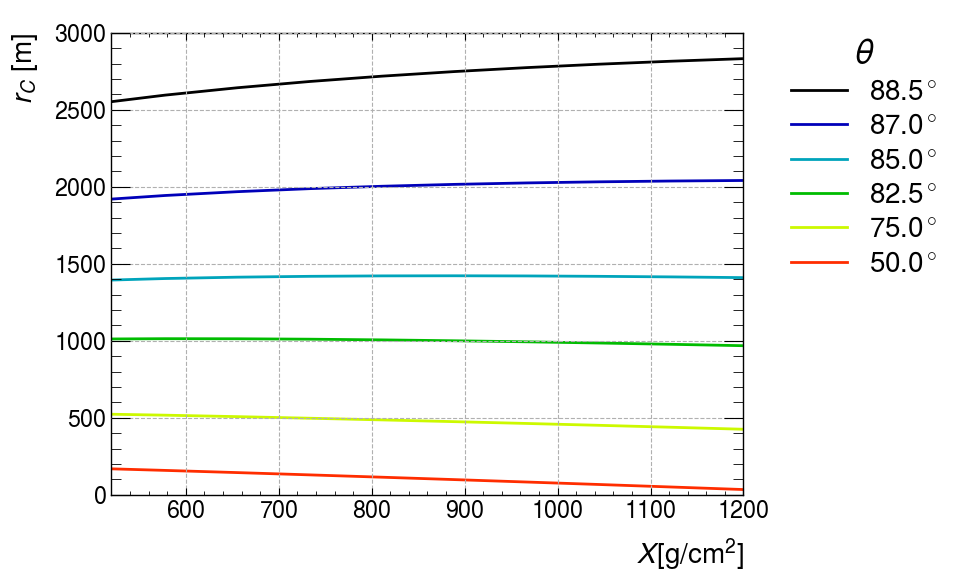
\includegraphics[width=0.5\textwidth]{gramm3}
    \caption{ The Cherenkov radius (\rc) as a function of slant depth (\x) for different zenith angles (\thet).}
    \label{fig:gramm3}
\end{figure}

The results displayed in Fig.~\ref{fig:gramm3} indicate a consistent decrease in \rc as \x increases for \thet less than 82\c. For \thet between 82.5\c and 86\c,  a single value of \rc can have two values of \x. This \thet region is also characterised by having a very minimal change in the value of \rc from a change in \x. In the case of \thet greater than 86\c, the footprint continuously increases as a function of \x. However, the rate of increase changes from shallow to deep slant depths;\ie the increase in the \rc range from 650\gr to 700\gr will be much larger than the change from 850\gr to 900\gr as can be seen in Fig. \label{fig:gramm3}.

%HS reviewed until here: May-2-2023


\subsection{ Impact of deviations in atmospheric depth on  \rc and \thet}\label{sec:2}
To investigate the impact of deviations in the measured slant depth \x on \rc and \thet, we focused on a single depth of 750\gr, which is close to the average \xmax recorded for showers above 10$^{19}$ \,EeV by the Pierre Auger Collaboration \cite{Aab_2014}. We introduced deviations of $\pm10$\gr, $\pm30$\gr, $\pm50$\gr, and $\pm100$\gr as a proxy for uncertainties in the slant depth measurement. We then calculated the corresponding deviation in \rc, denoted by $\Delta_r$, by working backwards from the deviations in \x.$\Delta_r$ is given by: 
\begin{equation}\label{del_r}
 \Delta_r(X,\Delta_X)=\frac{|(r(X+\Delta_X)-r(X)) + (r(X)-r(X-\Delta_X))|}{2}
\end{equation}
And zenith angle deviation, $\pm \Delta_\theta$ given by:
\begin{equation}\label{del_t}
\pm \Delta_\theta = |\theta(r_{750}\pm \Delta_r)-\theta(r_{750})|
\end{equation}
 This is shown graphically in Fig.\ref{fig:gramm5} and Fig. \ref{fig:gramm6}.

\begin{figure}[ht!]
    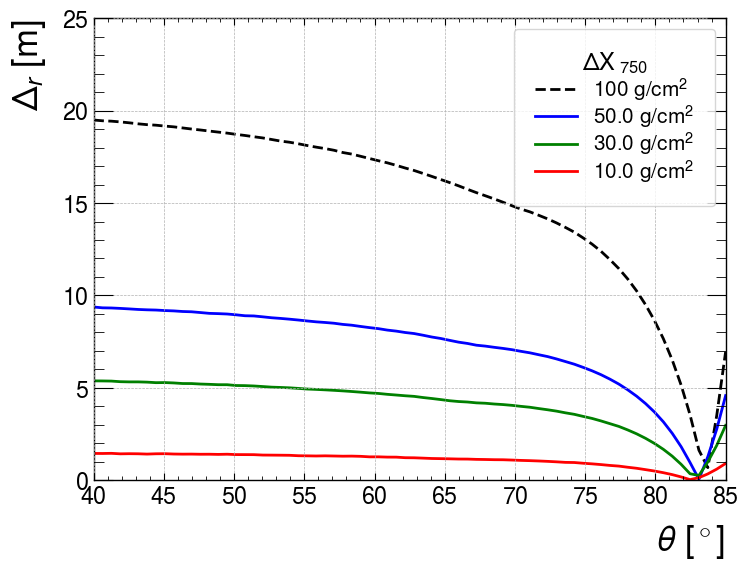
\includegraphics[width=0.47\textwidth]{gramm5}
    \caption{Deviations on  the cherenkov radius ($\Delta_r$) as a function of Zenith angle (\thet) for different deviations on \x = 750\gr.}
    \label{fig:gramm5}
\end{figure}
\begin{figure}[ht!]
    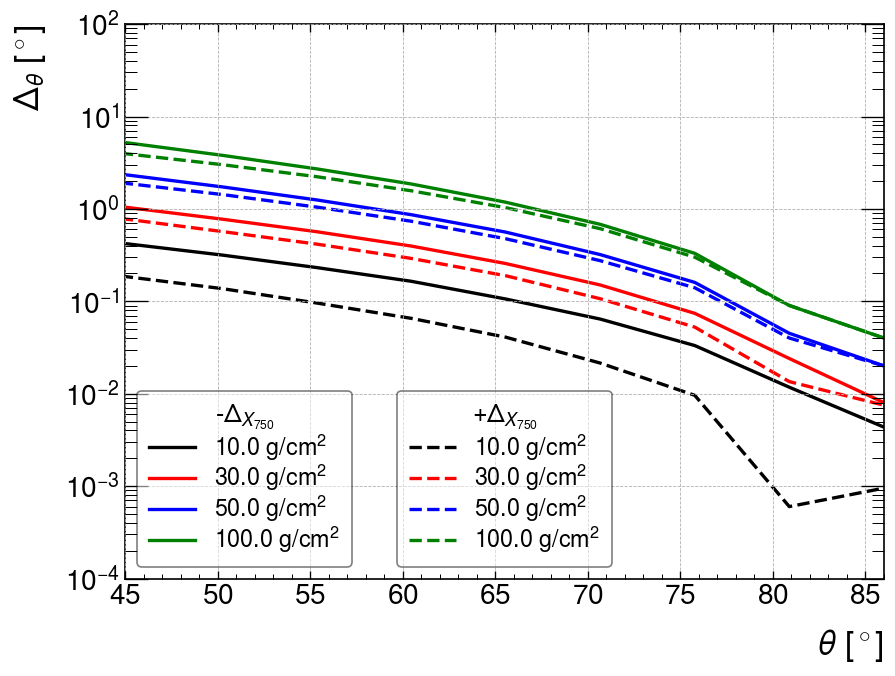
\includegraphics[width=0.47\textwidth]{gramm6}
    \caption{Deviations on zenith angle ($\Delta_\theta$) as a function of zenith angle (\thet) for different deviations on \x = 750\gr.}
    \label{fig:gramm6}
\end{figure}
Figure \ref{fig:gramm5} and \ref{fig:gramm6} show the deviations or resolution required on \rc and \thet respectively, to attain a $\pm$10\gr, $\pm$,30\gr,$\pm$ 50\gr and $\pm$100\gr deviation on an \x of 750\gr. The dips in Figure \ref{fig:gramm5} between 82.5\c and 84\c, indicate a minimal change in \rc at that value of \thet despite changes in \x. The figures can also be interpreted as; to achieve a resolution of $\pm$10\gr, we would require a resolution of \rc of $\pm2$\m for \thet $\leq$  75\c. We also observe a steepening in slope between 75\c and $\approx$ 82\c. This shows how strong the zenith dependence is on the footprint in this zenith region. Figure \ref{fig:gramm6}, shows the asymmetry in $\Delta_\theta$, $+\Delta_{X_{750}}$ and $-\Delta_{X_{750}}$ shows how strong the \rc dependence is with increasing \thet, as much smaller angles are required are to give the same change in \rc for the +$\Delta_{X_{750}}$ case as opposed to the -$\Delta_{X_{750}}$. We can also note that to archive a $\pm10$\gr on 750\gr would require a zenith angle accuracy of less than a thousandth of a degree for zenith angles greater than 80$^{\circ}$. For a $\Delta_\theta$ of $\pm$100\gr, this is less than a tenth of a degree in zenith angle reconstruction for zenith angles greater than 80\c.  

\subsection{A Special Angle}
In Fig. \ref{fig:gramm3}, shows a zenith angle region where the size of \rc with respect to \x remains nearly constant. After examining Fig.\ref{fig:gramm5}, we have identified this zenith angle region to start from approximately 82.85\c and end at 86\c for a U.S. standard atmosphere and ground altitude of 1425\,m. The lack of change in \rc is due to projection effects resulting from the signal being generated at a far distance from the ground, resulting in stretched emission cones over longer distances in the atmosphere than would be possible for vertical zenith angles, this is illustrated in Fig. \ref{fig:magic_L}. 

\begin{figure}[ht!]
\includegraphics[width=\linewidth]{MagicA.png}
\caption{The schematic illustrates the dependence of the Cherenkov radius (\rc) on the zenith angle (\thet). We present three zenith angle scenarios; $\theta << \theta_M$, $\theta = \theta_M$, and $\theta >> \theta_M$. each with two emitters having the same difference in slant depth ($X_E-X_B$). The distance with respect to the zenith angle increases to cover the same difference in slant depth (\x). For the case of $\theta_M$, we found that \rc remains constant for both $X_B$ and $X_E$}
\label{fig:magic_L}
\end{figure}
In Fig. \ref{fig:magic_L}, the increase in $n$ increases the $\psi_C$ increases with larger values of $n$, this causes the emission cones from deeper emitters ($\rm X_E$) to be slightly wider than those from shallow emitters (\rm $X_E$). When $\theta << \theta_M$ , both emitters are located relatively close to the ground. As a result, the shallower emitter \rc than the deeper emitter. When $\theta = \theta_M$, both emitters have the same \rc. This occurs because the effect of the source distances balances out with the broadening effect of $\psi_C$. For $\theta >> \theta_M$, the broader beam emitted by the source and the increased distance from the ground cause the deeper emitter to cover a larger \rc than the shallower showers. 


\section{Simulated air showers}\label{sec:sims}
To investigate if the findings in Sec.\ref{sec:1} could be observed in radio Monte Carlo radio simulations. We generated 60 simulations using  ZHAireS \cite{ZHAireS} version 1.0.30a. All simulations were composed of protons primaries with an energy of 1 EeV, and azimuth angle of 90\c in three discrete zenith angle bins i.e., 50\c, 82.85\c, and 88.5\c. The corresponding \rc values for a shower with an \xmax of 750\gr ($r_{C_{750}}$) to these zenith angles are 125\m, 1053\m  and 2690\m, respectively. Each simulation contained 20 antennas evenly distributed along a length of $\approx$ 4 $r_{C_{750}}$ for that particular \thet. The orientation of the antenna line was set perpendicular to the azimuthal direction of the incoming shower. We used a ground altitude of 1425\m and geomagnetic field parameters corresponding to the Pierre Auger observatory for all simulations, \ie an Intensity of 23.57$\,\mu$T, a magnetic inclination of -37.07\c and a declination of 0.52\c. SIBYLL23d \cite{Riehn2020} was the hadronic model utilised and applied a  relative thinning of $10^{-5}$. From the 20 showers in each zenith angle set, 6 events were selected, these showers roughly covered an \xmax range from $\approx$ 660\gr to $\approx$ 1050\gr.

\section{\xmax dependence on the distribution of the Maximum Amplitudes}
\label{sec:ldf}
The lateral distribution of the maximum amplitude of the electric field against the antenna distance w.r.t. the shower core. This is a useful tool used in estimating \rc which can be used to determine \xmax \cite{LOFARNATURE}. The point of maximum amplitude in the distribution corresponds to \rc given by Eq. \ref{eq:01}. In Fig.\ref{fig:LDFamps} We calculated the maximum amplitude in both the Pierre Auger observatory  (30--80\,MHz)\cite{2018JCAP...10..026A}  and GRAND (50--200\,MHz)\cite{2020SCPMA..6319501A}  frequency bands in the $\vec{v} \times \vec{B}$ polarisation, which corresponds to the polarisation direction from the geomagnetic emission of the shower. The effects of changing the band can be seen from the right (a,c,e) to left (b,d,f) plots in Figure \ref{fig:LDFamps}. The narrow 30--80\,MHz band gives much smoother distributions with amplitudes $\approx$ 3 times less than those of the broader 50--200\,MHz band. The higher amplitudes in the 50--200\,MHz band exhibited sharper features than those of the narrower band. This can be observed by the prominence of the plateau-like humps indicative of the Cherenkov ring, which can easily be distinguished up to an \xmax $\approx$ 950\gr in image (b) in comparison to (a) of Figure \ref{fig:LDFamps}.

\begin{figure*}[h!]
\centering
\begin{tabular}{cc}
    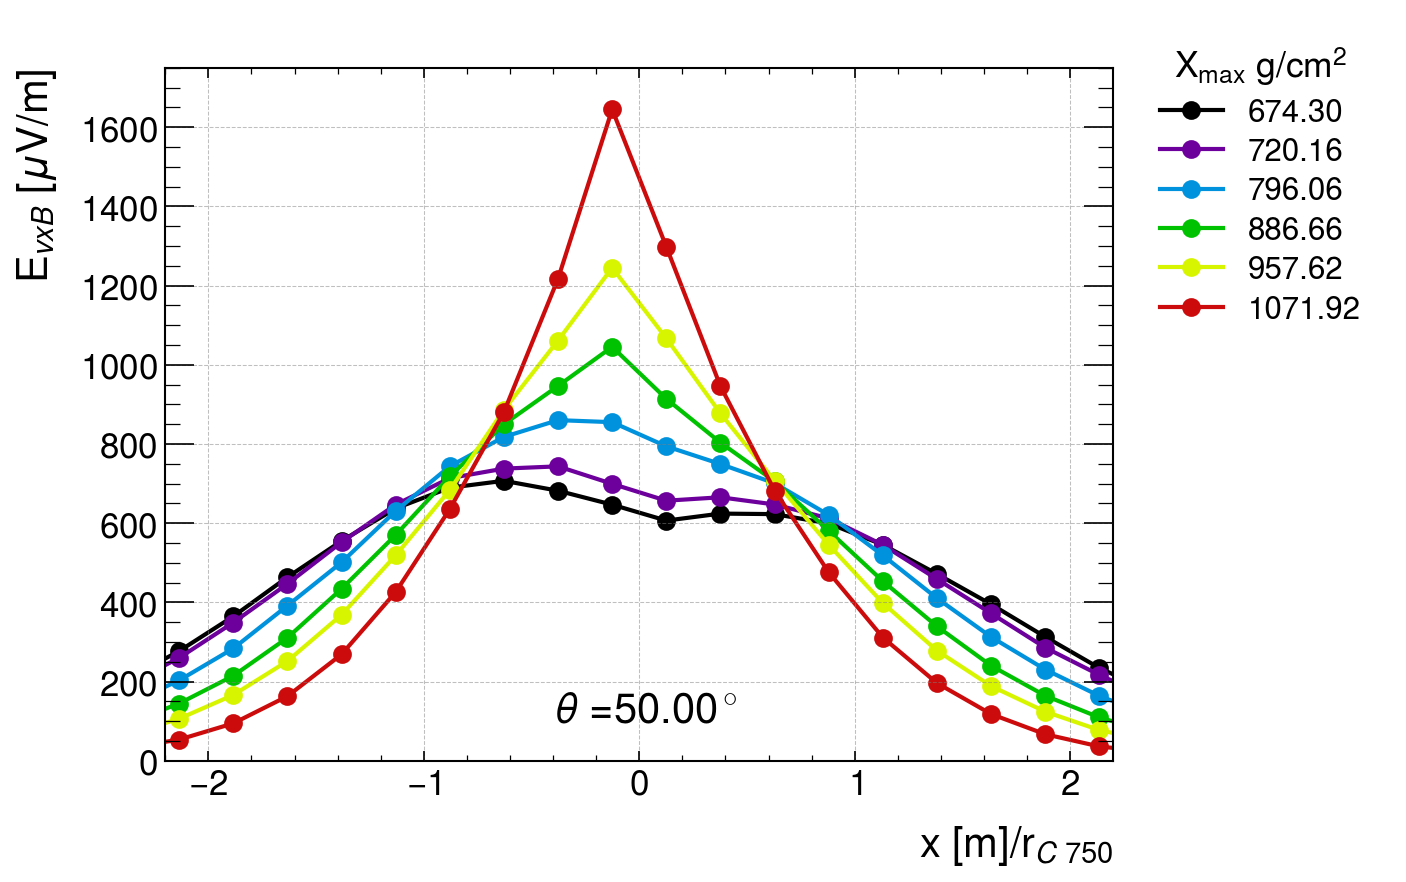
\includegraphics[width=0.45\linewidth]{50zenLDF.png} &
    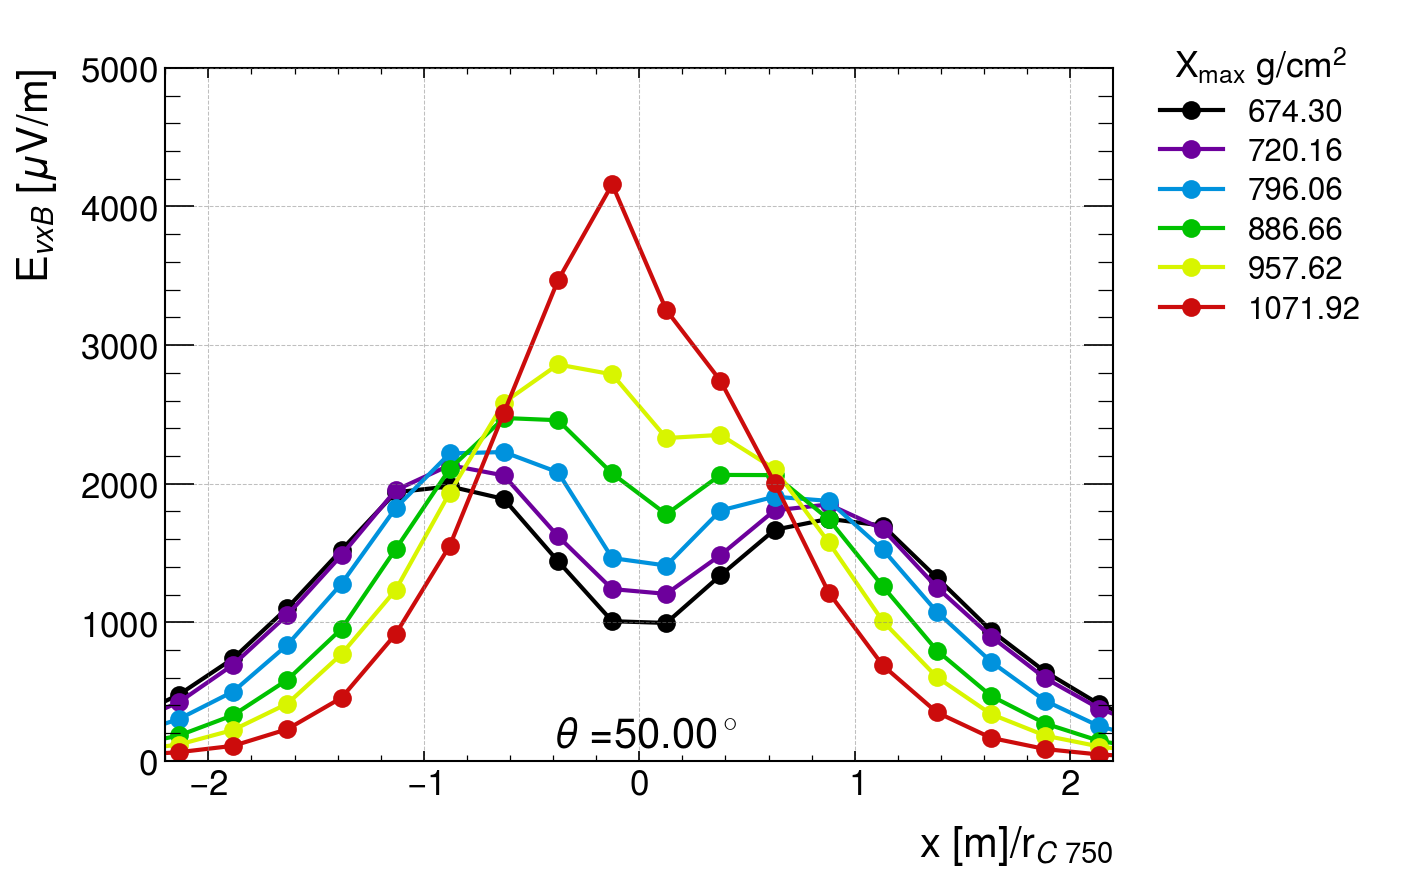
\includegraphics[width=0.45\linewidth]{50zenLDF200.png} \\
    \textbf{(a)} & \textbf{(b)} \\
    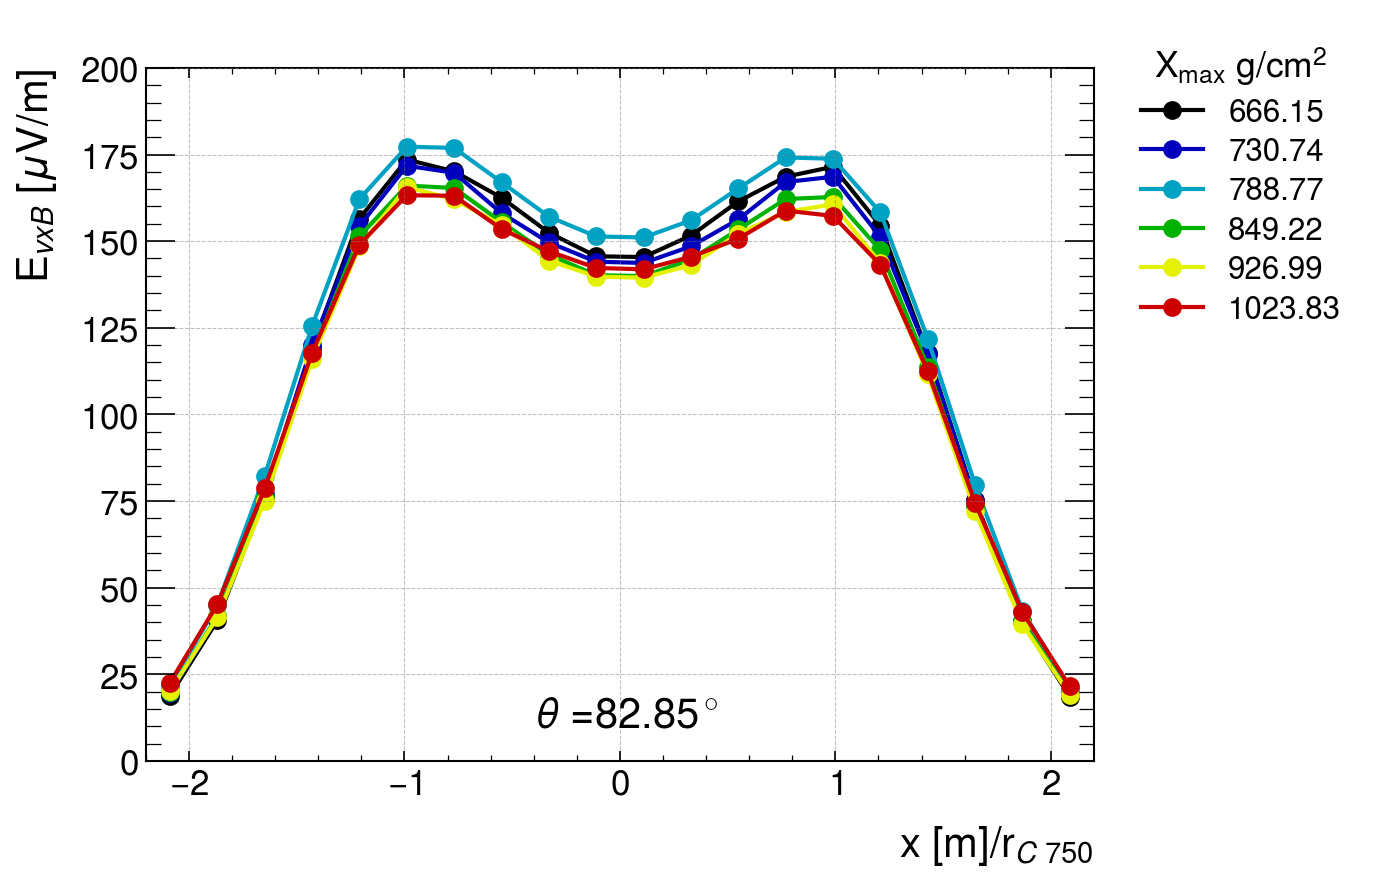
\includegraphics[width=0.45\linewidth]{82zenLDF.png} &
    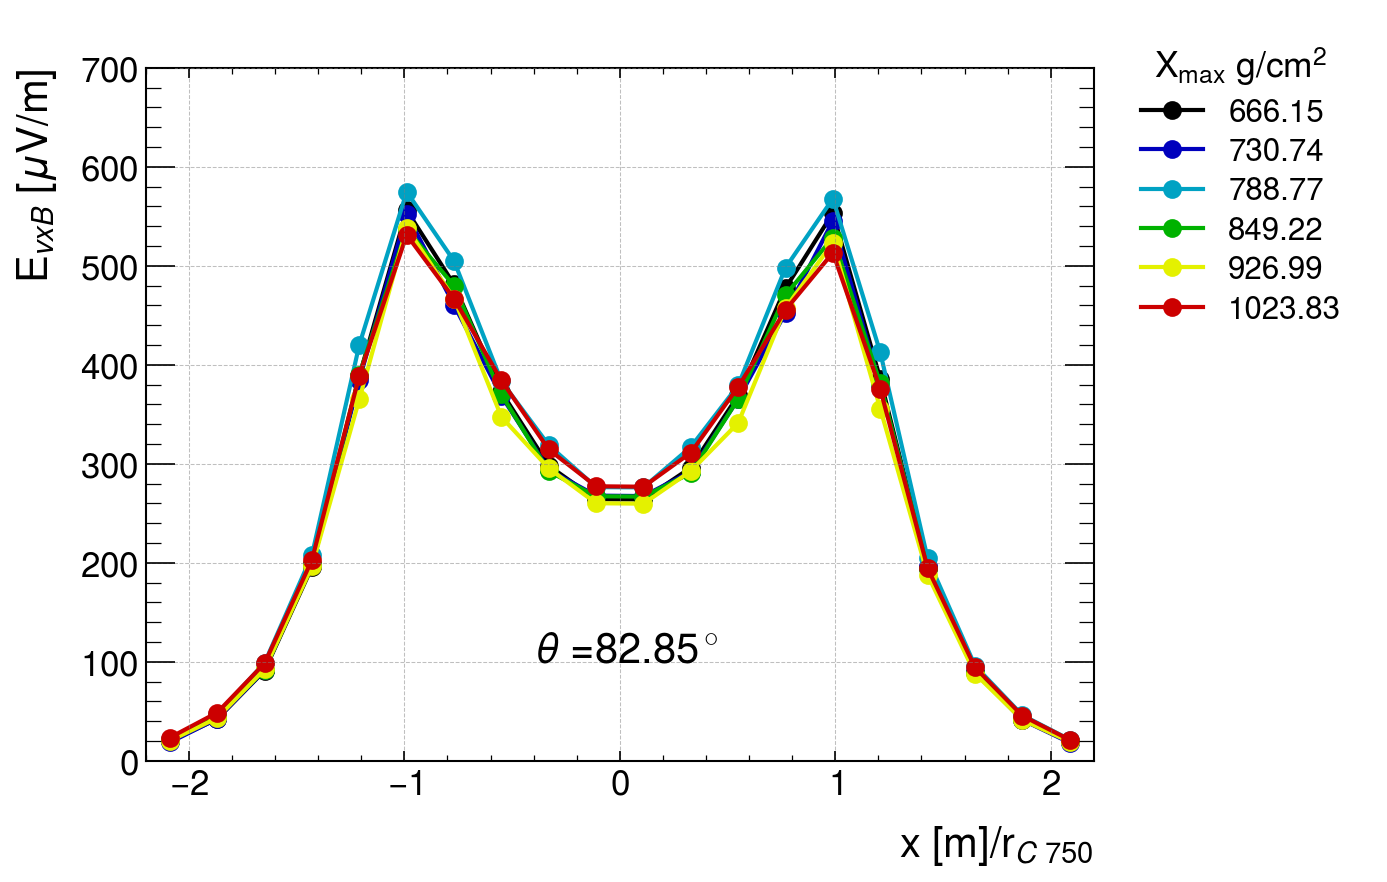
\includegraphics[width=0.45\linewidth]{82zenLDF200.png} \\
    \textbf{(c)} & \textbf{(d)} \\
    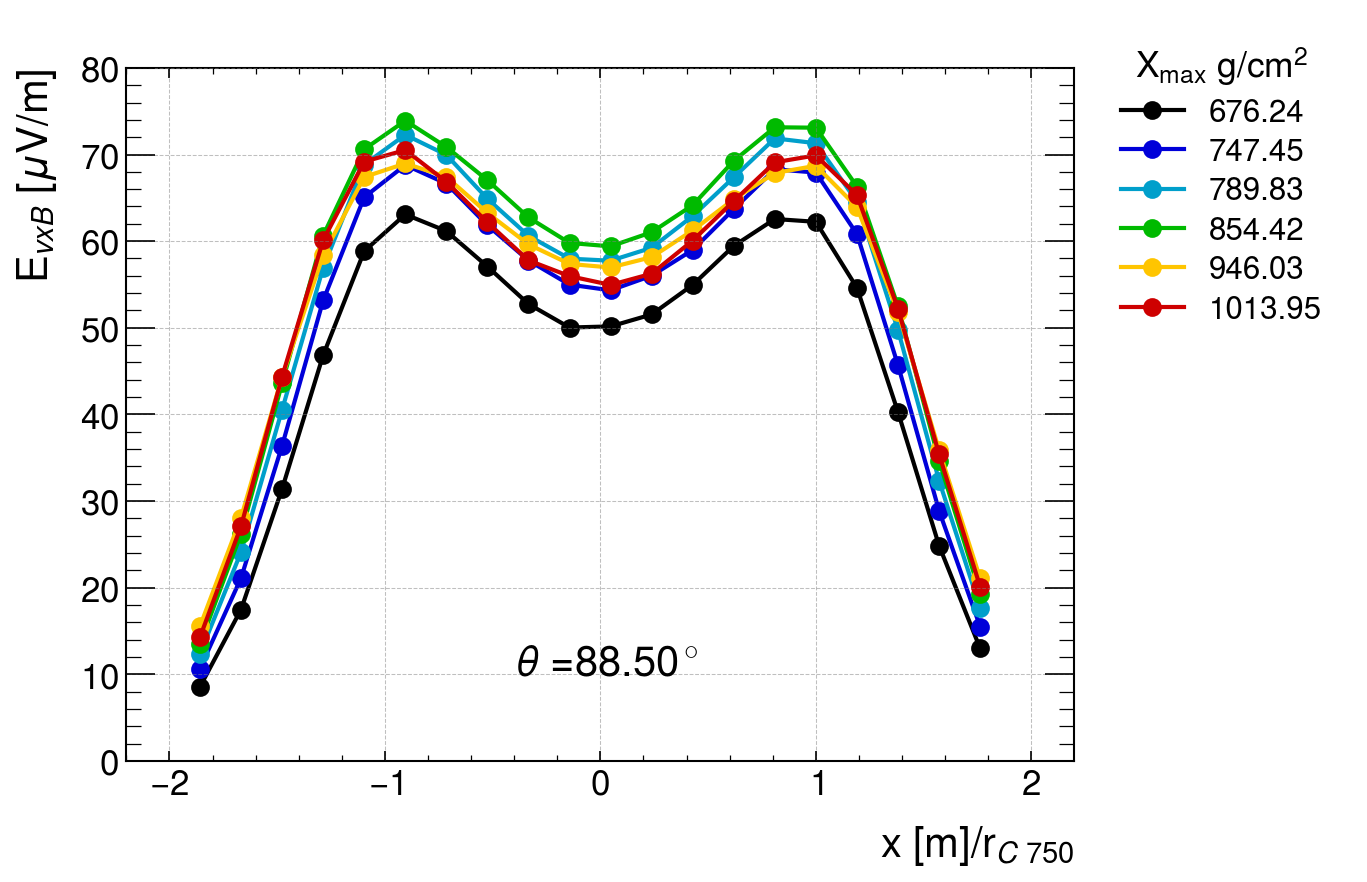
\includegraphics[width=0.45\linewidth]{88zenLDF.png} &
    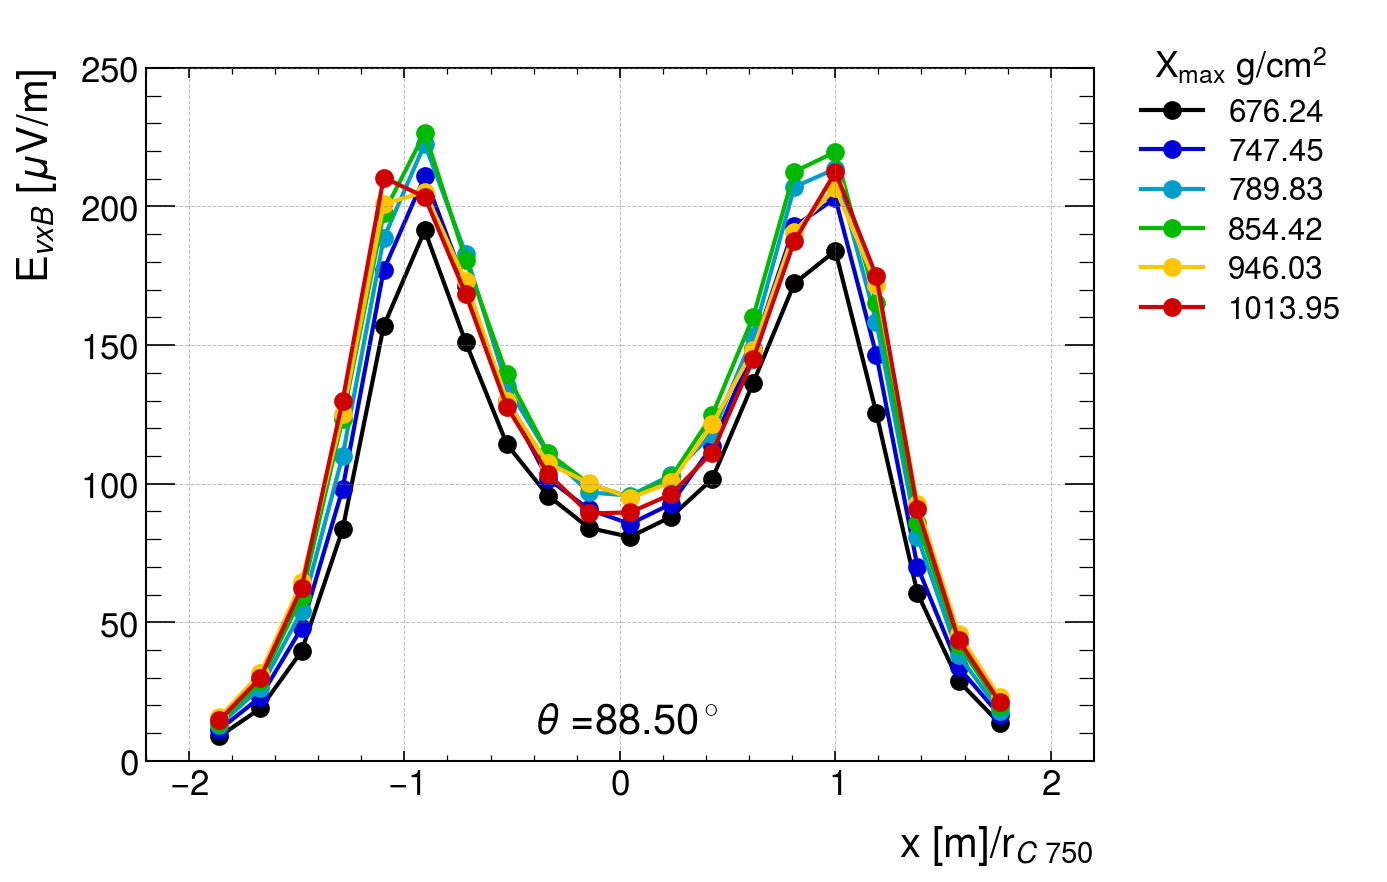
\includegraphics[width=0.45\linewidth]{88zenLDF200.png} \\
\textbf{(e)} & \textbf{(f)} \\
\end{tabular}
\caption{Images (a,c,e); distribution of amplitudes in the frequency band 30\,MHz--80\,MHz. Images (b,d,f); the LDF in the 50\,MHz--200\,MHz frequency band for different \xmax. }
\label{fig:LDFamps}
\end{figure*}

Plots (a) and (b) in Fig. \ref{fig:LDFamps} demonstrate the \xmax dependence from the distribution at a zenith angle of 50\c. We observe that deeper and shallow showers have different shapes, and the width of the distribution increases with a reduction in \xmax. This changes for very inclined showers, as depicted for the 88.5\c case, where shallower showers are seen to have narrower distributions than deep showers, with the shape of the distribution being identical. The amplitudes of the distributions in the 88.5\c are also greatly reduced owing to the signal traversing great distances through the atmosphere(\ie 1/r dependence). The \xmax ordering is present, but we expect added complexity to the signal brought about by a change in the radio emission mechanisms for showers developing in a less dense atmosphere \cite{}. At 82.85\c, there is no discernable ordering of \xmax as the width and general shape of the distributions are roughly the same, as depicted in images (c) and (d). All three cases agree with the scenarios sketched in Fig. \ref{fig:magic_L}.

\section{\xmax dependency of the spectral shape distribution}
\label{sec:slope}
Figure \ref{fig:spectra} shows the frequency spectrum of different antennas w.r.t to the antenna distance to the shower core. 
\begin{figure*}[ht]
    \centering
    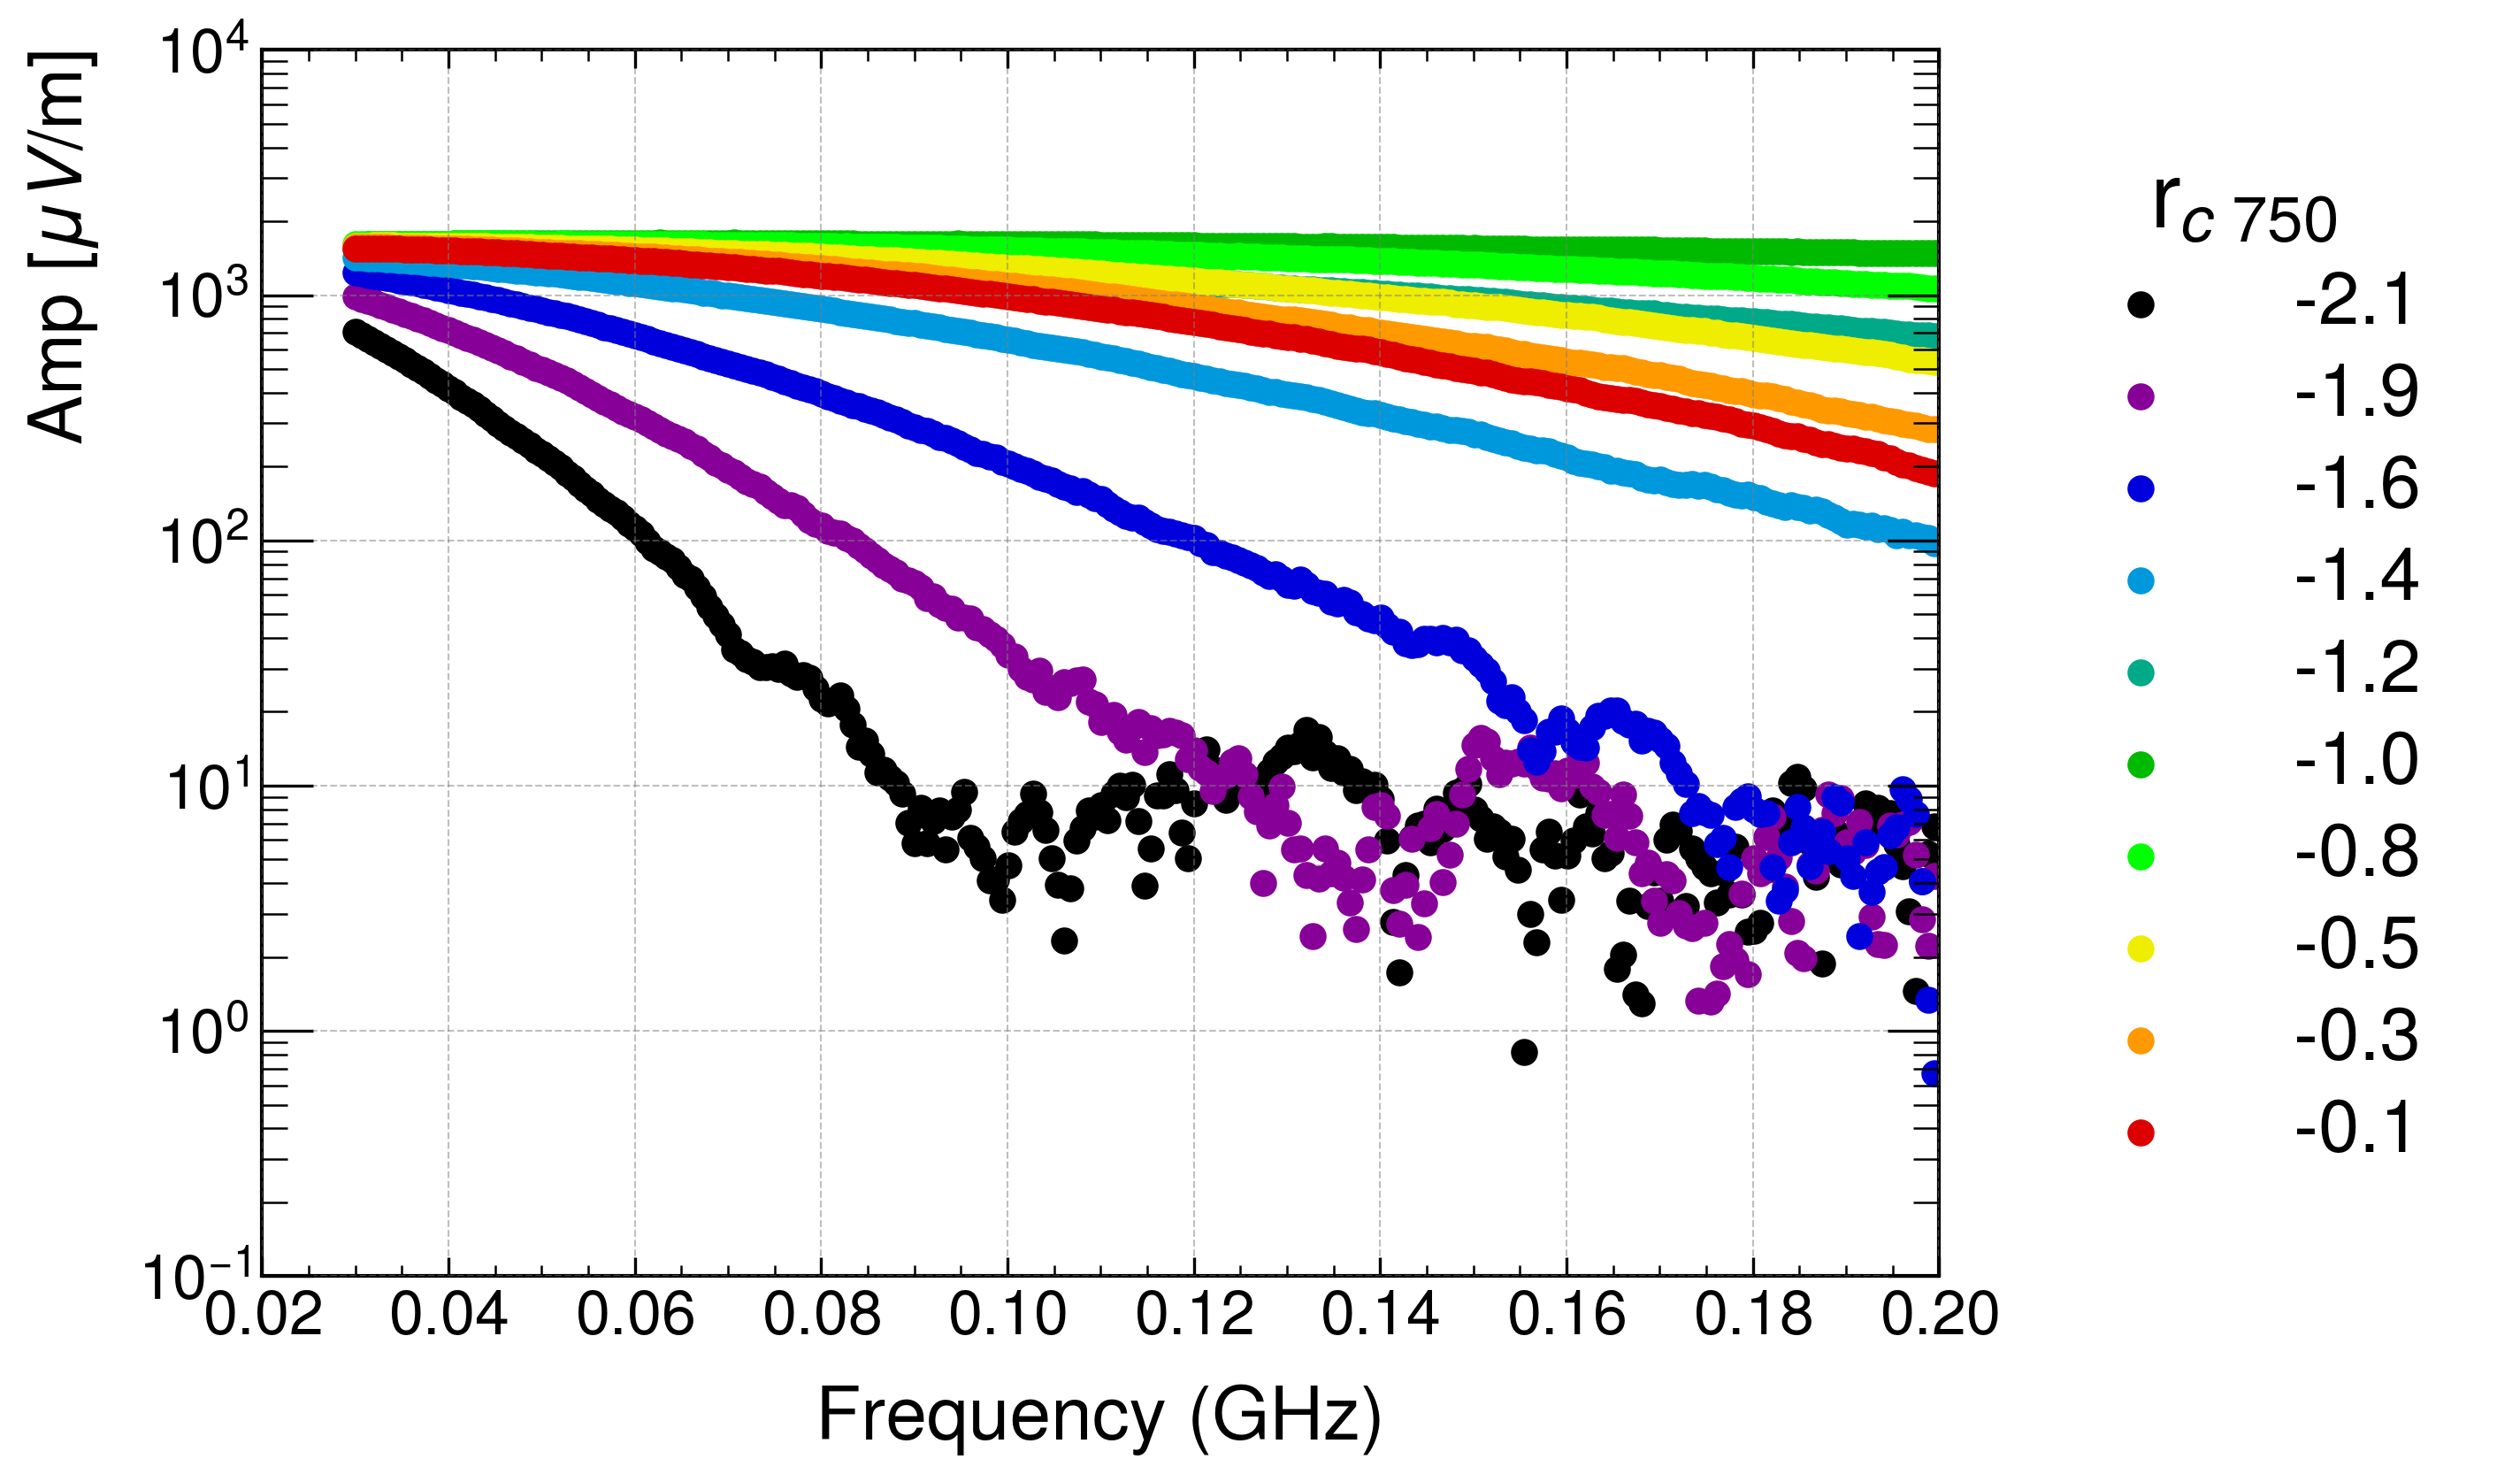
\includegraphics[width=.5\linewidth]{spectra2}\hfill
    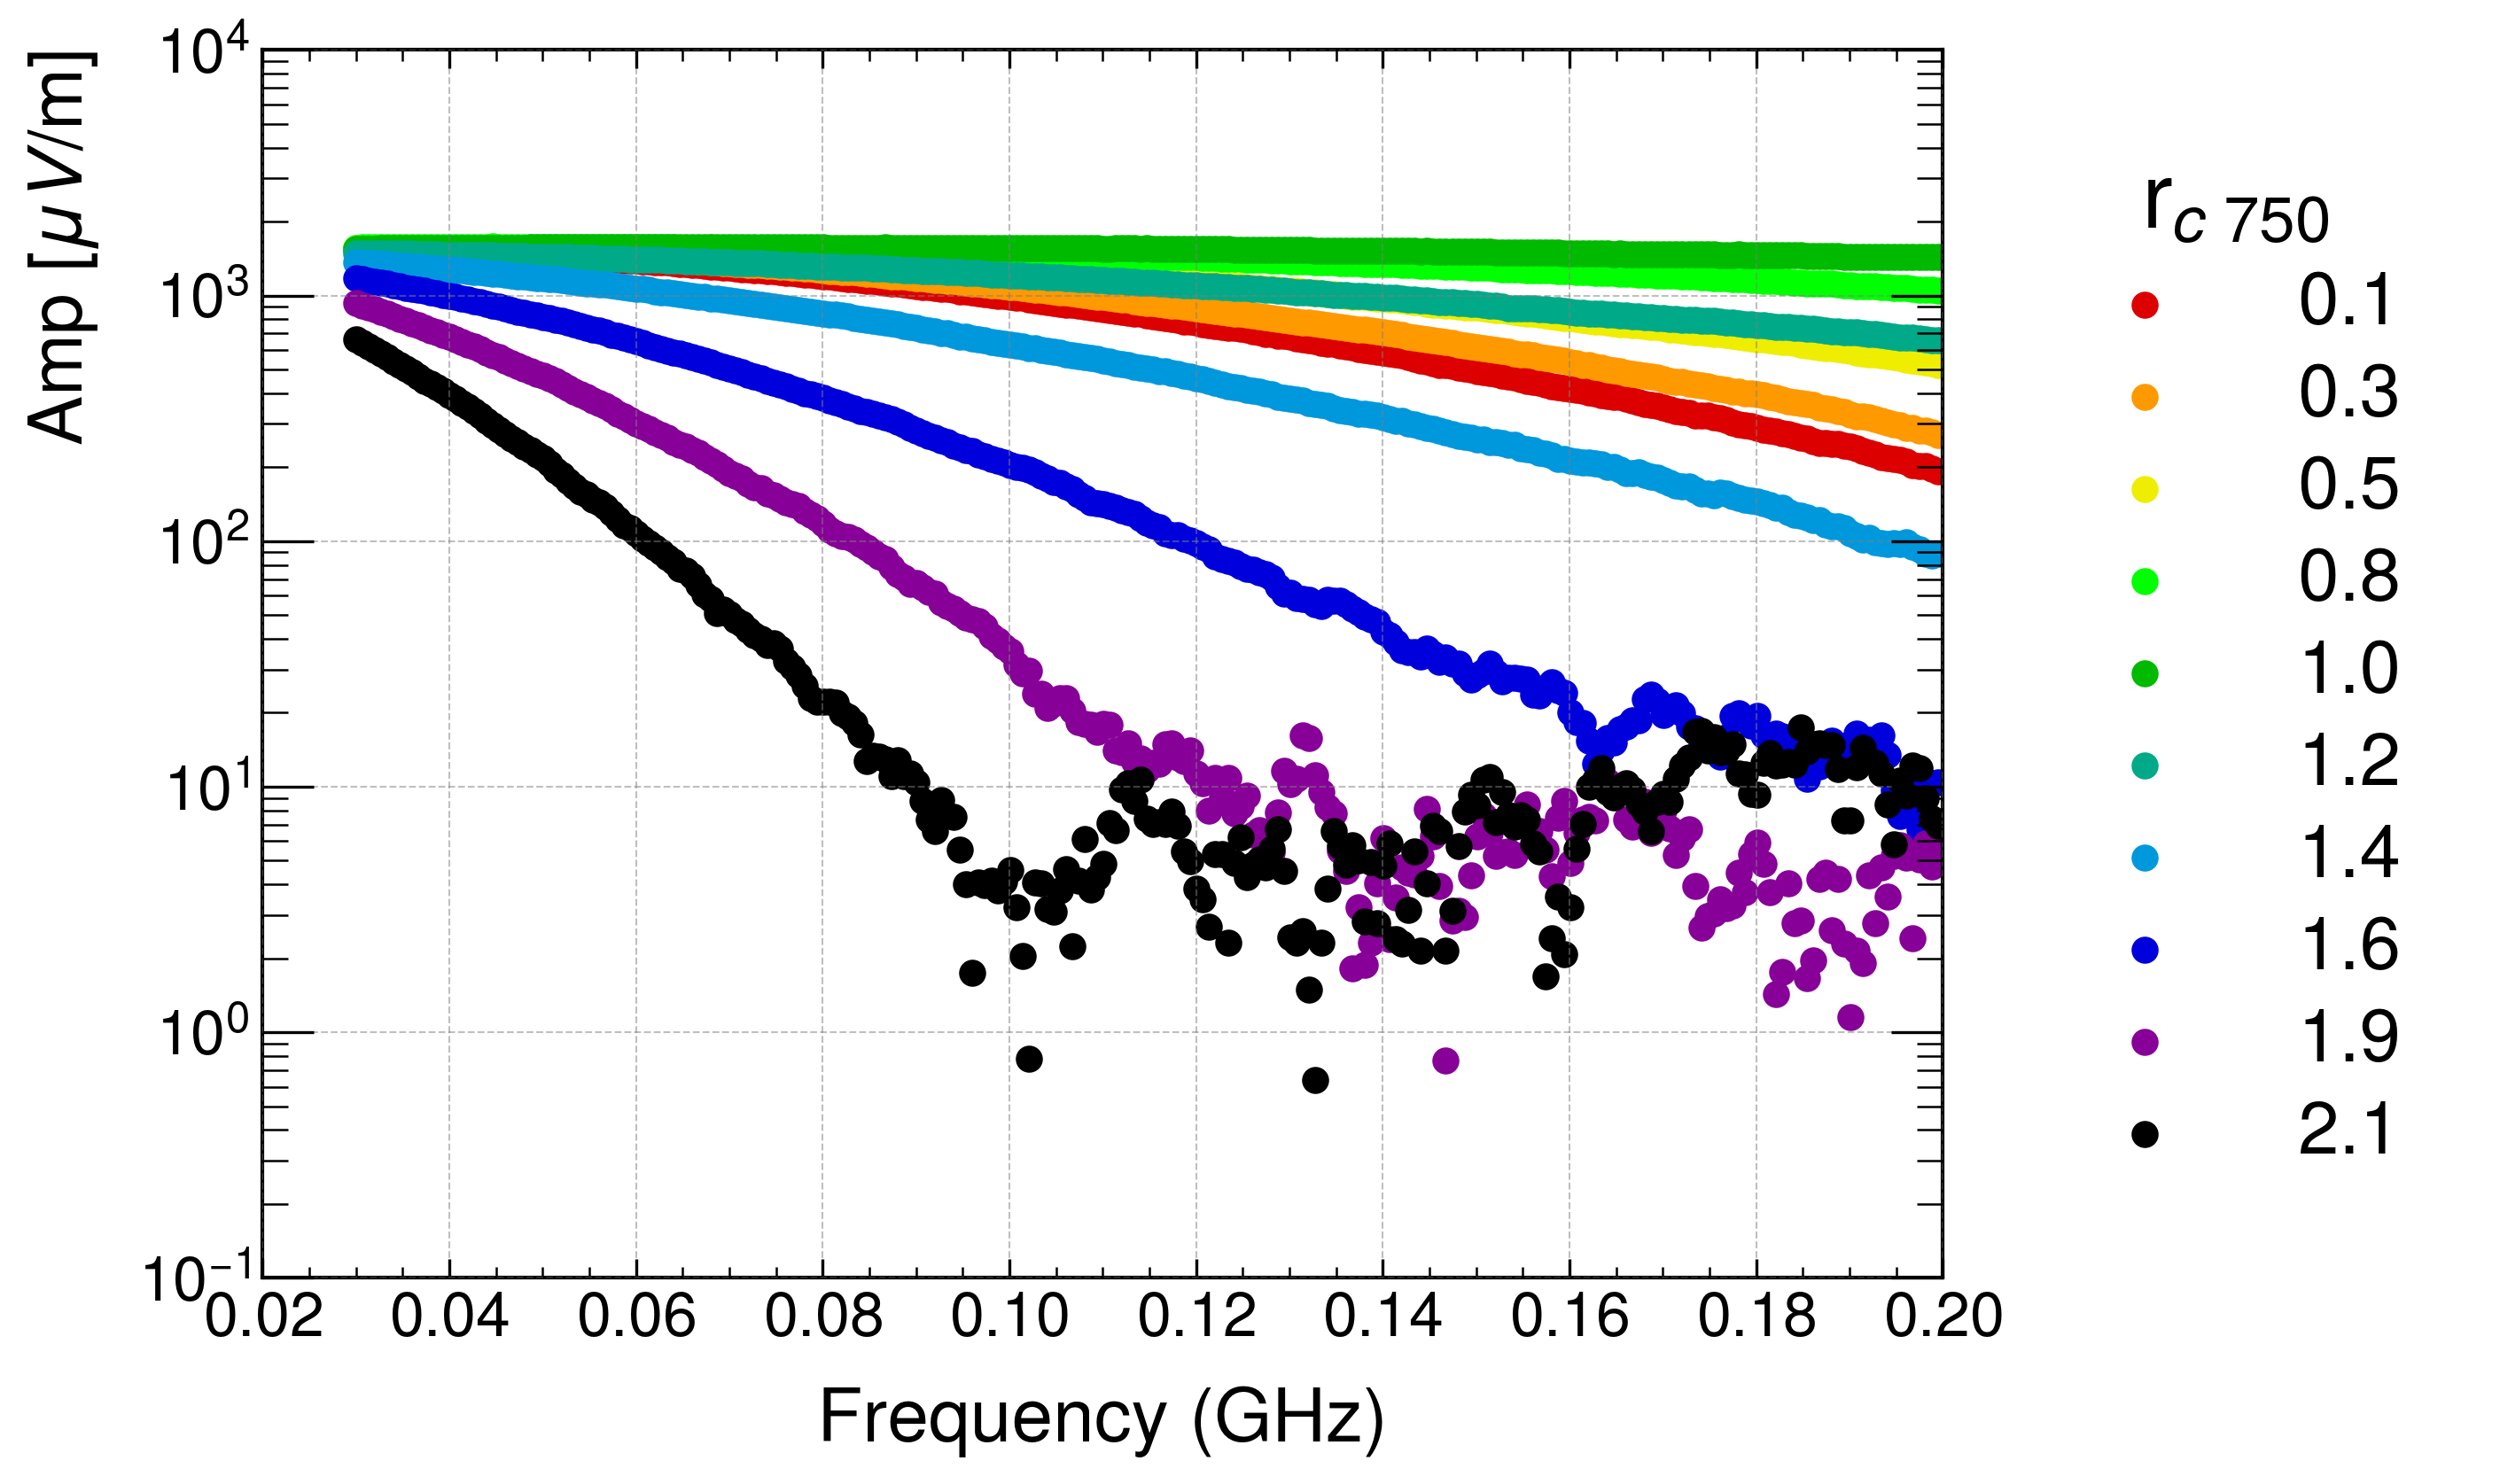
\includegraphics[width=.5\linewidth]{spectra}
    \caption{The frequency spectrum as a function of antenna distance from shower core.}
    \label{fig:spectra}
\end{figure*}
As the distance from \rc increases, the slope of the frequency spectrum of the detected signal decreases. This change in slope is a result of the broadening of the pulse as a function of distance from the Cherenkov ring. At \rc, the fast pulse in the time-domain approaches a delta-function, resulting in a flat amplitude in the frequency domain, as illustrated in Fig.\ref{fig:spectra}. To determine the spectral index, we first determine the spectral slope by fitting a polynomial to the amplitude of the frequency domain, given by Eq. \ref{eq:01}:
\begin{equation}\label{eq:01}
S(\nu-\nu_0)= a_1(\nu-\nu_0)^2+ a_2(\nu-\nu_0)+a_3
\end{equation}
Here, $S$ represents the amplitude of the signal as a function of frequency, with $\nu_0$ denoting a reference frequency or slope frequency and the coefficients $a_1$, $a_2$, and $a_3$ fit parameters. Evaluating the derivative of Eq.\ref{eq:01} at $\nu_0$ yields the spectral slope. To obtain the spectral index, we normalise the evaluated slope by the spectral amplitude at the slope frequency, as shown in Eq. \ref{eq:02}.
\begin{equation}\label{eq:02}
    b  \coloneqq \frac{1}{\ln(10)\cdot S(\nu-\nu_0)} \left(\frac{d}{d\nu}S(\nu-\nu_0)\right)\biggr\rvert_{\nu_0}=\frac{a_2}{\ln(10)\cdot a_3}
\end{equation}
$S(\nu-\nu_0)$ represents any well-fitting function to the frequency domain, given by  Eq. \ref{eq:01} in our case, and $\nu _0$ is the slope frequency. This formulation of the spectral index is equivalent to previous analyses that obtained the spectral index as one of the coefficients of the fit equation: $S(\nu-\nu_0)=10^{b(\nu-\nu_0) + c}$ to the frequency spectrum \cite{Jansen:2016sjo}. The spectral index $b$ characterises the pulse shape, reducing signal amplitude dependence. 
Figure \ref{fig:indx_dist} shows the distributions of the spectral index as a function of antenna distance to the shower core obtained at $\nu_0=$ 50\,MHz and $\nu_0=$150\,MHz.To get rid of antennas with thinning artefacts in our analysis, we applied a filter to remove antennas with low signal, which was determined by a threshold equal to 5 times the median value of the amplitudes for frequencies greater than 100\,MHz of the two antennas located at the edges of the antenna line.
\begin{figure*}[th!]
\centering
\begin{tabular}{cc}
    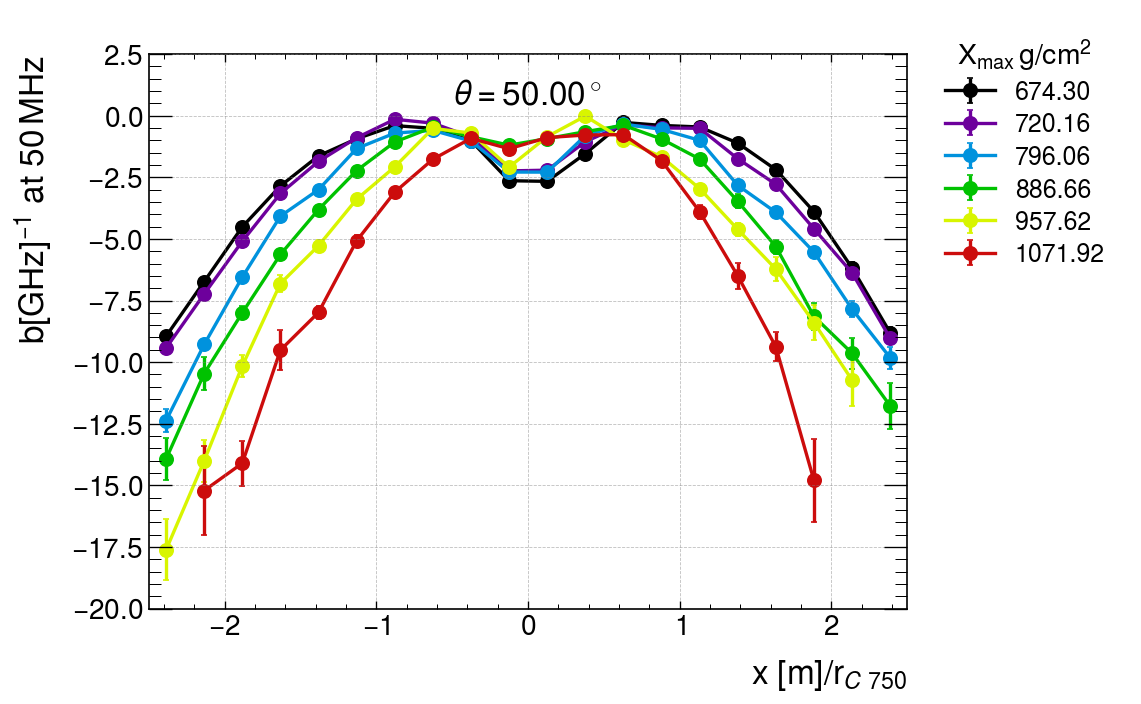
\includegraphics[width=0.45\linewidth]{spec_Indx50_50.png} &
    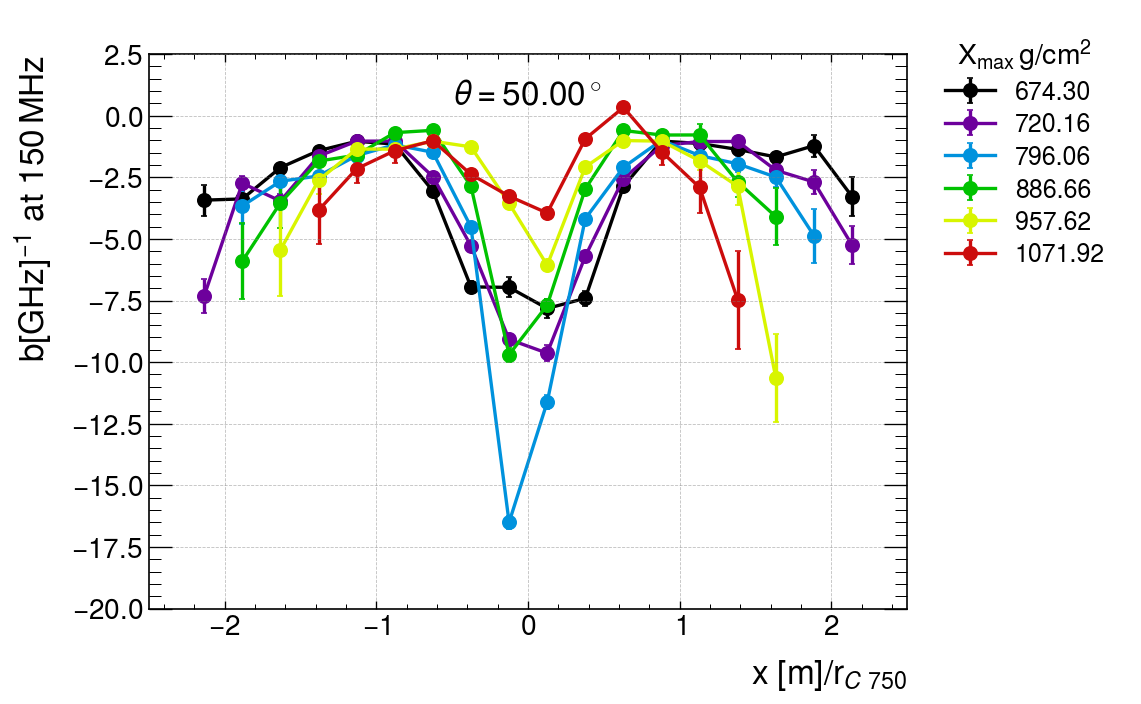
\includegraphics[width=0.45\linewidth]{spec_Indx50_150.png}\\
    \textbf{(a)} & \textbf{(b)} \\
    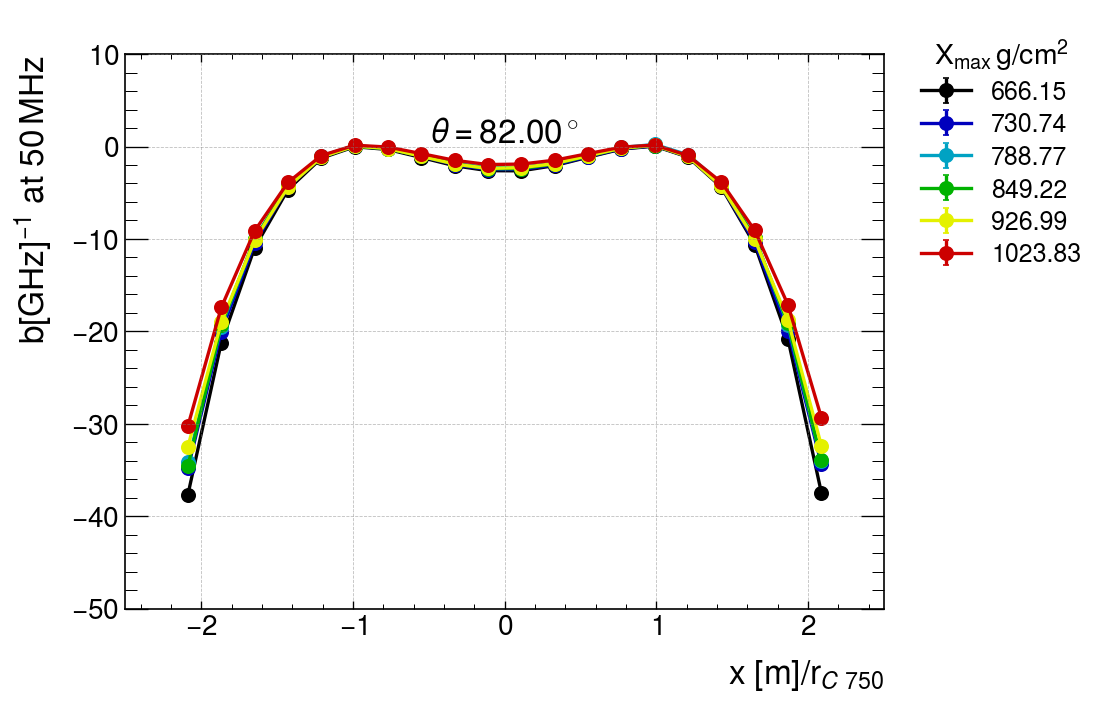
\includegraphics[width=0.45\linewidth]{spec_Indx82_50.png}&
    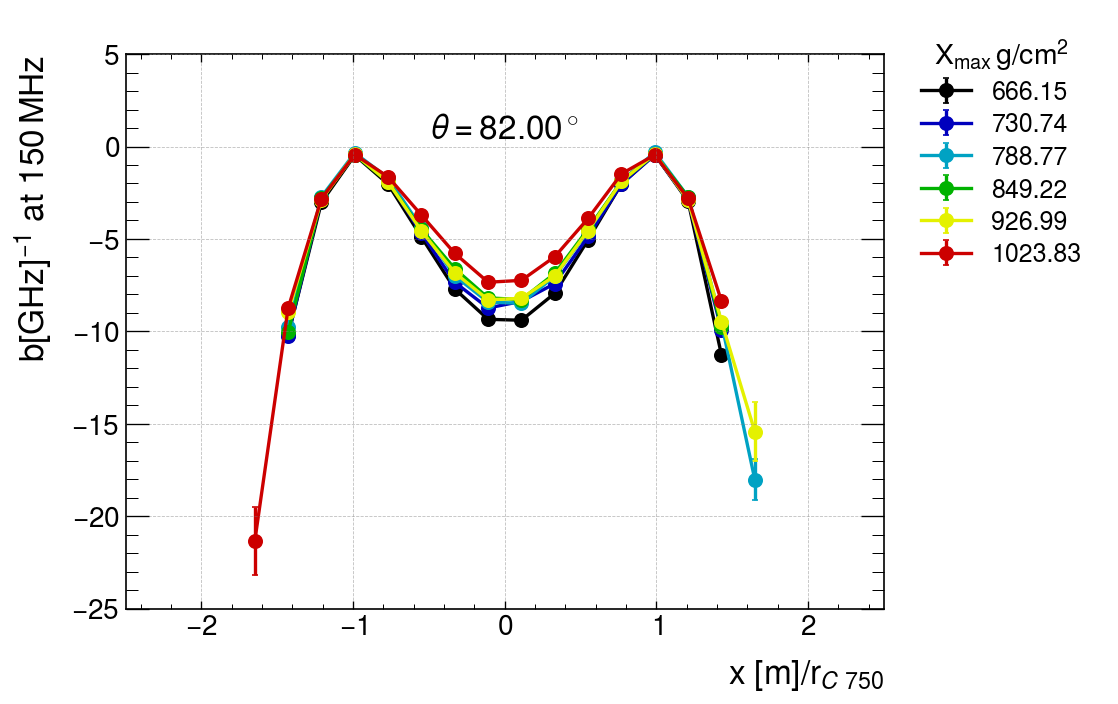
\includegraphics[width=0.45\linewidth]{spec_Indx82_150.png}\\
    \textbf{(c)} & \textbf{(d)} \\
    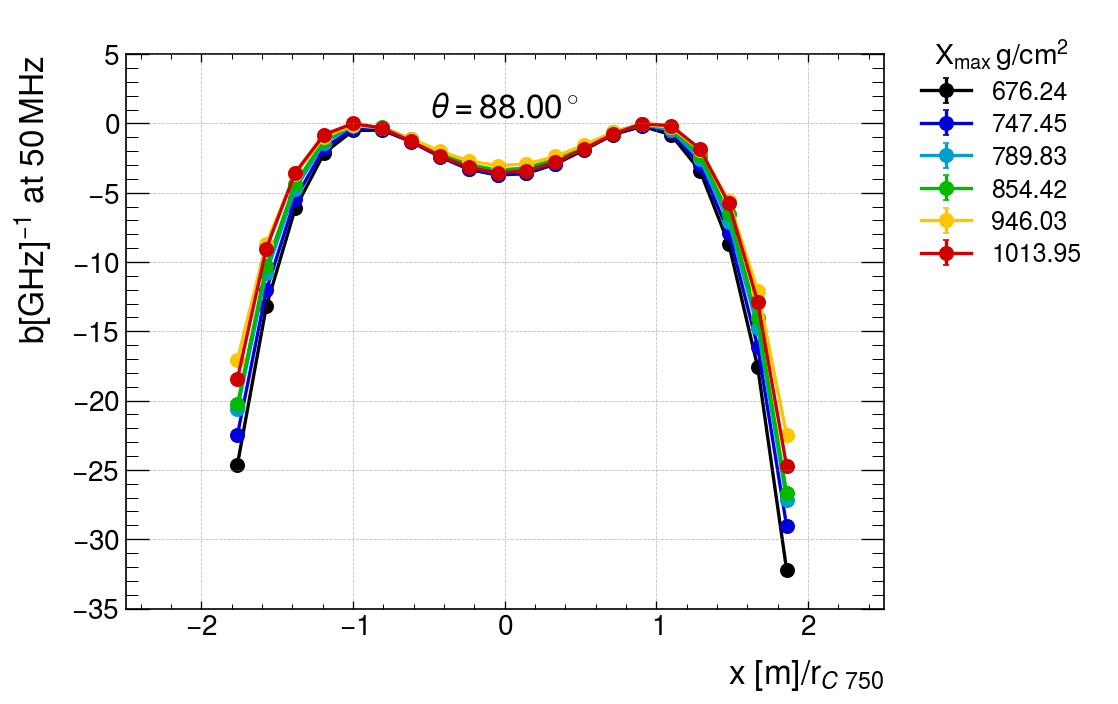
\includegraphics[width=0.45\linewidth]{spec_Indx88_50.png} &
    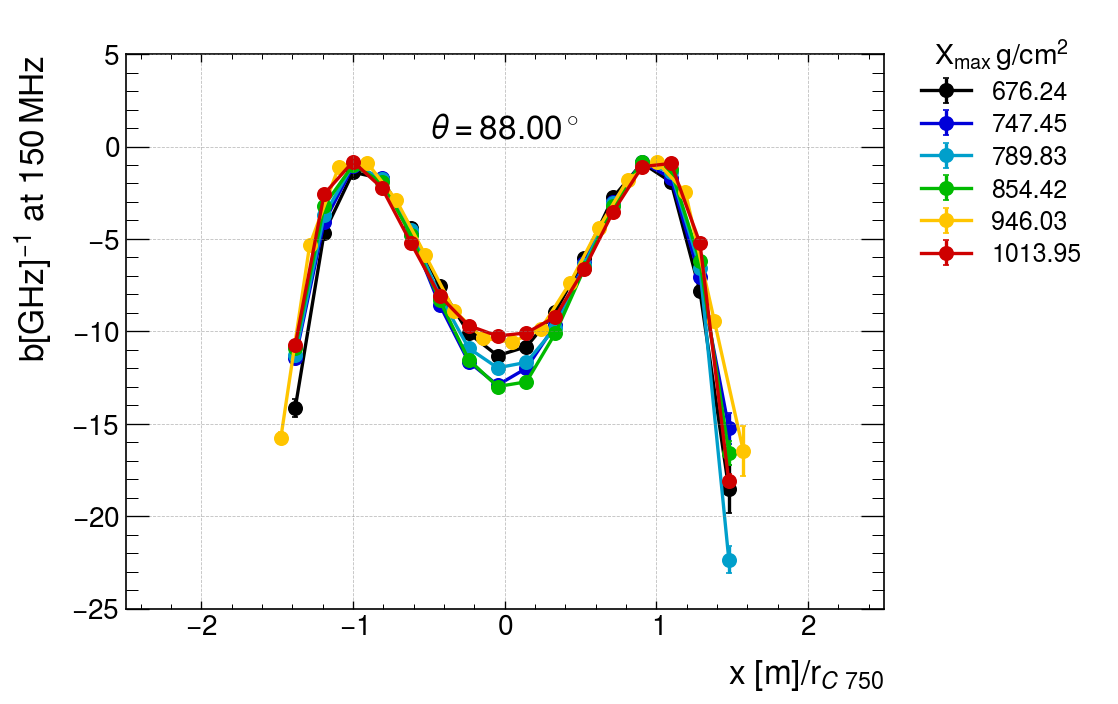
\includegraphics[width=0.45\linewidth]{spec_Indx88_150.png}  \\
\textbf{(e)} & \textbf{(f)} \\
\end{tabular}
\caption{The spectral index distribution for varying \xmax at slope frequencies of 50 MHz (a,c,e) and 150MHz (b,d,f).}
\label{fig:indx_dist}
\end{figure*}
In Fig.\ref{fig:indx_dist}, we observe that the lower slope frequency gives a much smoother distribution with a very clear \xmax dependence. The spectral index for $\nu_0=$ 50\,MHz shows \xmax ordering at distances $\ge$ 1 \rc for the 50\c and 88.5\c cases, with the notable difference being the inversion of the \xmax ordering.This is similar to our observations in the distribution of amplitudes and slopes. The higher slope frequency has very prominent bumps at \rc but the distributions have no discernable \xmax dependency, especially for the inclined cases. For the 82.85\c case, the ordering in \xmax starts at around 1.5\rc with no visible fluctuations at \rc.
\\In both the distribution of maximum amplitudes and spectral indices, the \xmax dependency of the two distributions can be seen to invert from low to high zenith angles. However, both distributions do not give any discernable change on the \rc as a function of \xmax at 82.85\c. Thus, \xmax measurements done in the 82\c--86\c range would require an alternative method.
 
\section{\xmax Dependency from interferometry}\label{sec:rit}

To evaluate the potential of interferometry in resolving the \xmax in the region where the amplitude distribution and spectral slopes had minimal sensitivity \ie at a zenith angle of 82.85\c, we created a second set of simulations to be used for the Radio Interferometric Technique (RIT) \cite{Schoorlemmer2021}. The simulation set consisted of  160 antennas arranged on a hexagonal grid with a spacing of 1.5\,km and another set at 1\,km to resemble the Pierre Auger Observatory's and GRAND setups, respectively. All other inputs for the simulations remained similar to the simulation set discussed in Sec. \ref{sec:sims}.\\
The RIT technique has been demonstrated to reconstruct the direction and \xmax by utilizing coherent sums of the radio signals arriving at different antennas in the array. The use of interferometry in sparse array setups is especially possible at high zenith angles because the radio footprints become large enough to cover a sufficient number of baselines. Figure \ref{fig:xrit} shows the normalised integrated power in the transverse plane of the shower, the longitudinal integrated power as a function of slant depth \x and the correlation plot of the RIT reconstructed \xmax against the simulated \xmax. The reconstruction in these plots assumes ideal synchronisation, \ie having zero timing uncertainties between antennas. 

\begin{figure*}
    \centering
    \begin{tabular}{ccc}
 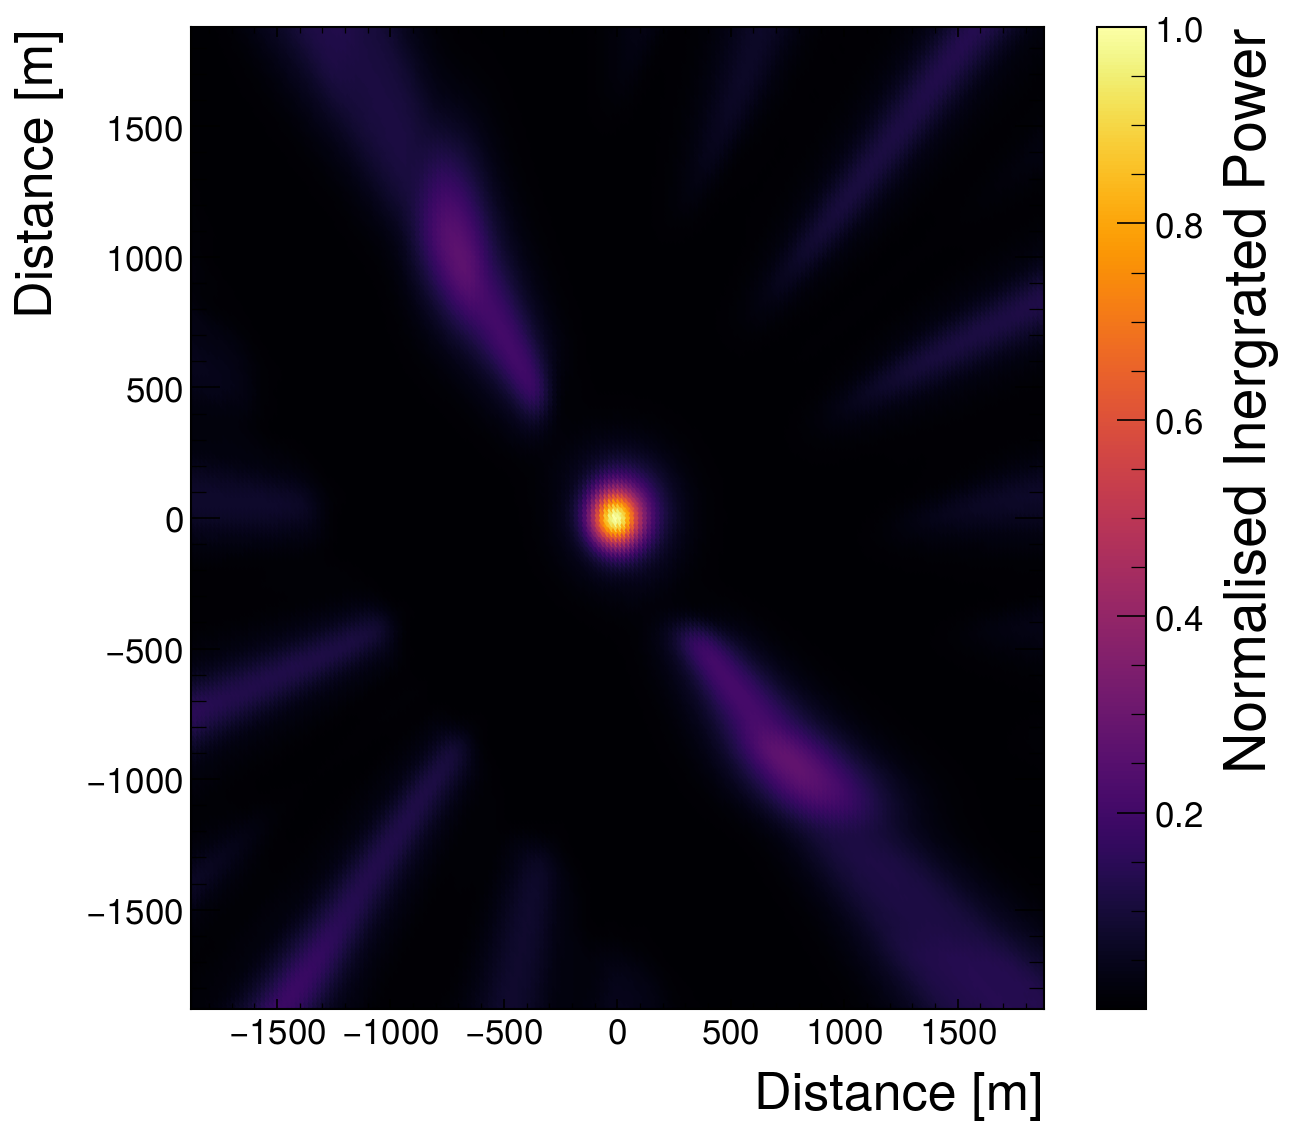
\includegraphics[width=0.3\textwidth]{plt_axis.png} & 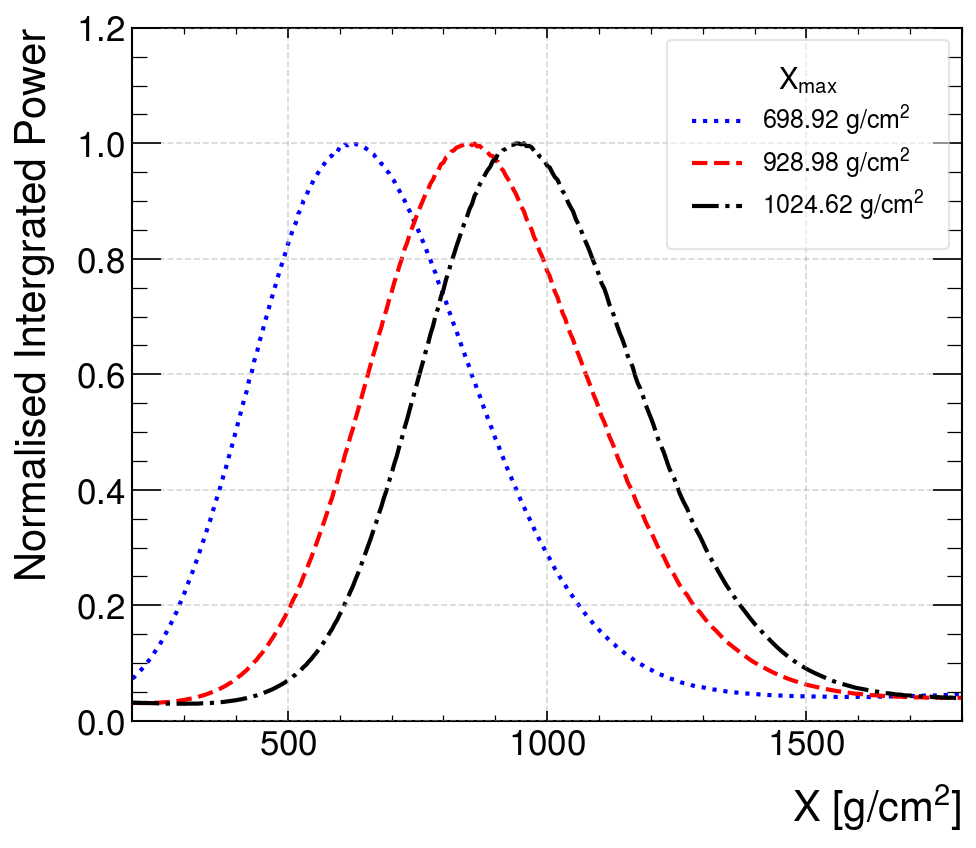
\includegraphics[width=0.3\textwidth]{long_pow.png} & 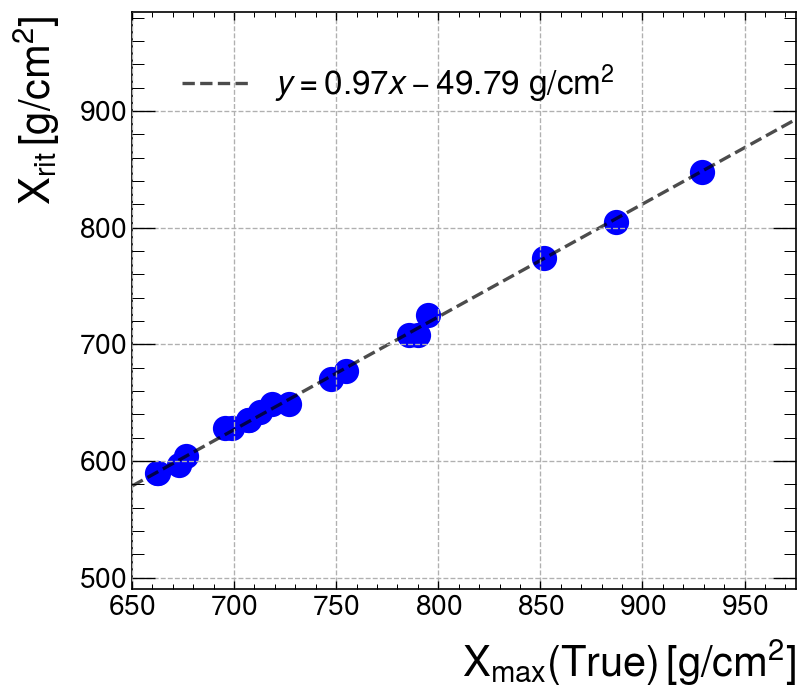
\includegraphics[width=0.3\textwidth]{XvXrit.png}  \\
 
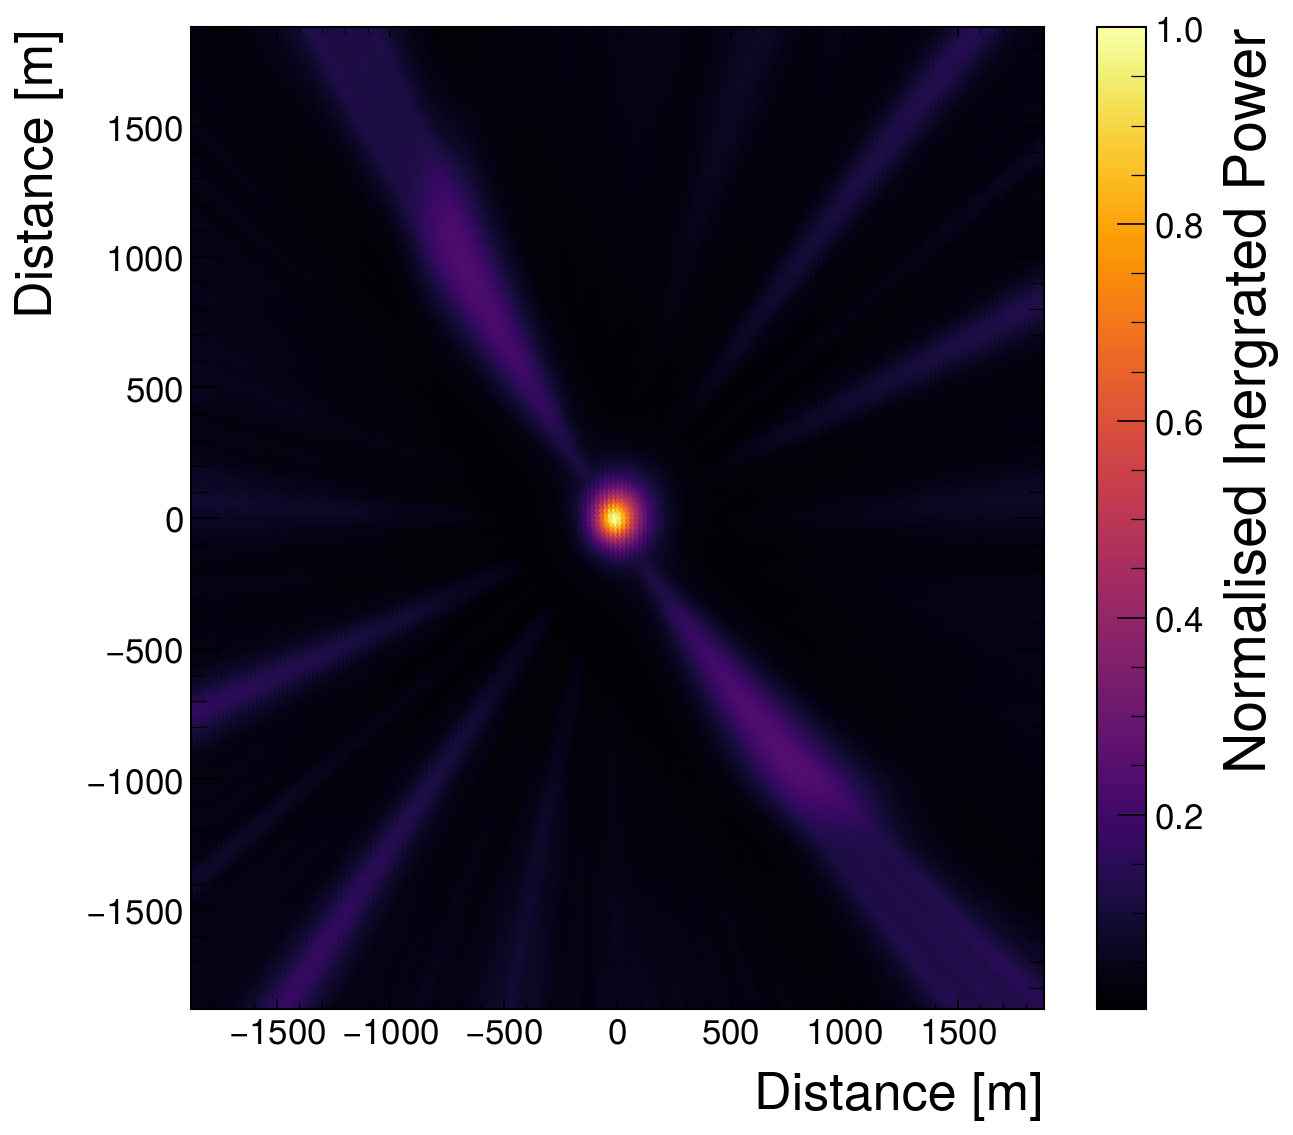
\includegraphics[width=0.3\textwidth]{plt_axis_200.png} & 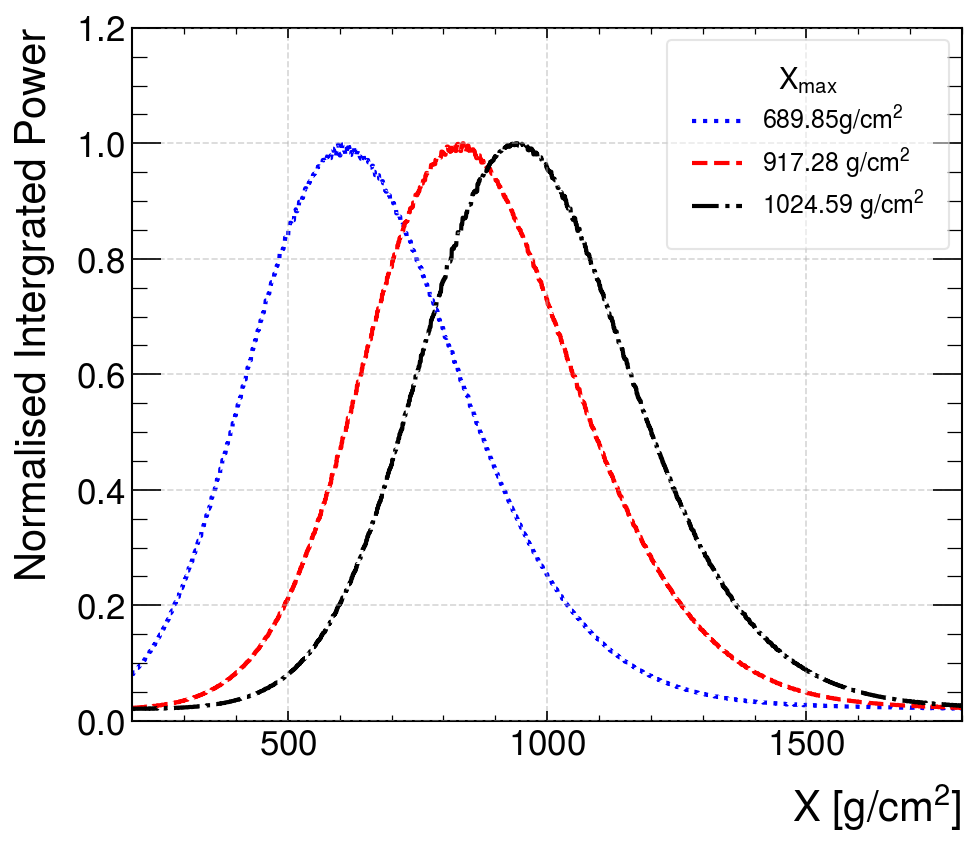
\includegraphics[width=0.3\textwidth]{long_pow_grand.png} & 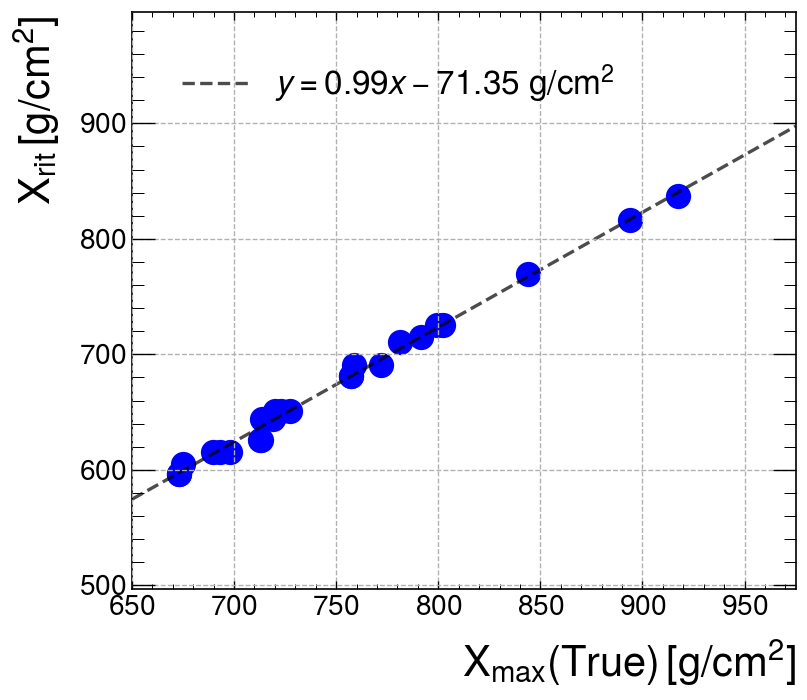
\includegraphics[width=0.3\textwidth]{XvXrit_2.png} \\        
         \textbf{a} & \textbf{b} & \textbf{c}
    \end{tabular}
    \caption{(a) A transverse slice of the atmosphere showing the integrated power at an atmospheric depth of 750\gr in the shower plane. (b) A plot illustrates the normalized power against the slant depth \x for three simulated showers. The power in images (a) and (b) is normalised by the maximum power. (c) A correlation plot comparing the true \xmax with the RIT reconstructed \xmax (\xrit) at a zenith angle of 82.85 degrees. The reconstruction was performed without any timing jitter or noise. The top images correspond to the frequency range of 30-80\,MHz with an antenna spacing of 1500\,m, while the bottom images correspond to the frequency range of 30-200\,MHz with an antenna spacing of 1000\,m.}
    \label{fig:grid}
\end{figure*}


To investigate how timing uncertainties affect the performance of \xmax reconstruction, we added different levels of Gaussian timing uncertainties to the time traces of the simulations and performed the reconstruction. The results in Fig. \ref{fig:rit_rms} show $\rm \sigma_{X_{max}}$calculated as Root-mean-square (RMS) of the reconstructed \xmax (\xrit) values plotted against the timing uncertainty $\sigma_t$.  

\begin{figure}[ht!]
    \centering
    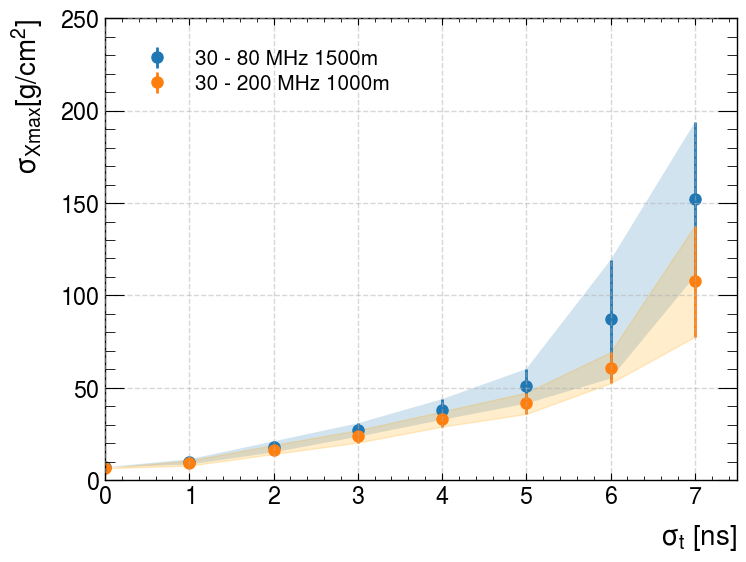
\includegraphics[width=0.5\textwidth]{rms_rita2.png}   
    \caption{Uncertainties in \xmax ($\rm \sigma_{X_{max}}$) as a function of the timing uncertainty $\sigma_t$.}
    \label{fig:rit_rms}
\end{figure}
As shown in Fig. \ref{fig:rit_rms}, for timing uncertainties within 5\,ns, there is a notable linear correlation between \xrit and the simulated \xmax. However, beyond 5\, ns of timing jitter, the accuracy of the reconstruction quickly diminishes as you lose coherency. This lack of coherency above a quarter wavelength. It is worth emphasizing that the RMS logarithmically scales with the timing uncertainty. This logarithmic scaling signifies that higher levels of timing uncertainty exert a more substantial influence on the accuracy of the \xrit.

\section{Discussion}\label{sec:disc}

In sections \ref {sec:ldf} and \ref{sec:slope} we demonstrated the use of the \rc as a measurement for the maximum shower depth. However, we have also identified limitations of methods reliant on \rc and the radio footprint in general. Specifically, in sparse array setups, to achieve a $\pm$ 10\gr resolution on shower maximum requires a resolution of $\pm$2 m on \rc and angular resolution of $\pm$0.001\c for zenith angles greater than 80\c. Both these values are beyond the accuracies currently attainable for sparse setups. 
\\
As demonstrated, both the LDF of the amplitudes and the slope distribution have sensitivity for estimating \xmax at \thet $< 82^\circ$ and $> 86^\circ$. But in the region 82\c$<\theta<$86\c, both these methods lose sensitivity to shower depth, as the dependence of \rc on shower depth transitions from flat to parabolic.

However, using interferometry, the size of the \rc only helps cover baselines that are later used in the coherent sum. For which, even at the extreme case of  82.85\c, the number of baselines is adequate for high-precision measurements of \xmax even with several nanoseconds of jitter. It's also worth noting that the addition of jitter to interferometric reconstruction reduces the resolution on the depth shower maximum from $\approx \pm$ 5\gr for sub-nanosecond jitter, to  $\approx \pm$ 100\gr for $\approx $ 6\,ns jitter. Above this level of jitter, the method loses coherency in the signal and can reconstruct neither the direction nor the shower depth, as shown in Fig.\ref{fig:rit_rms}. The combination of jitter, noise, and trigger thresholds is left for future studies.\\

The constant values of \rc and the footprint at the ''magic angle'' can provide an effective scaling of the electromagnetic energy to the particle energy, which will be useful in the calibration of the energy reconstruction of radio arrays.\\
A significant limitation of the radio interferometric technique is that, for an antenna spacing of $\approx$ 1,/km, the reconstruction may only be applicable for zenith angles above 70\c, as lower zenith angles reduce the number of baselines. This could be complemented by incorporating other techniques, such as the slope method, to improve the measurement of \xmax.

\section{Conclusion}\label{sec:conc}
Overall, the study shows the methods and limitations of utilizing the \rc to infer the shower maximum for inclined air showers. However, utilizing the radio interferometric technique would greatly enhance sparse arrays' mass detection sensitivity and capacity. On the other hand, how well this method performs will be subject to the accuracy of the timing synchronisation.

\begin{acknowledgements}
We would like to acknowledge the use of the C\&CZ in the Faculty of Science at  Radboud University. The high-performance computing resources provided by this facility were essential in carrying out the complex simulations and data analyses presented in this article. 
\end{acknowledgements}
\bibliographystyle{spphys} 
\bibliography{references.bib}% Produces the bibliography via BibTeX.

\end{document}


